\documentclass[12pt]{amsart}

% Packages
\usepackage{amsmath, amssymb, amsthm}
\usepackage{geometry}
\usepackage{hyperref}
\usepackage{cleveref}
\usepackage{graphicx}
\usepackage{enumitem}
\usepackage{color}
\usepackage{mathtools}
\usepackage{tikz}
\usepackage{tikz-cd}
\usepackage{quiver}
\usepackage{mathrsfs}

% Page Setup
\geometry{letterpaper, margin=1in}
\setlength{\parindent}{0pt} % No indent for paragraphs
\setlength{\parskip}{1em}   % Spacing between paragraphs

% Theorem Styles
\newtheorem{theorem}{Theorem}[section]
\newtheorem{lemma}[theorem]{Lemma}
\newtheorem{proposition}[theorem]{Proposition}
\newtheorem{corollary}[theorem]{Corollary}
\theoremstyle{definition}
\newtheorem{definition}[theorem]{Definition}
\newtheorem{example}[theorem]{Example}
\newtheorem{remark}[theorem]{Remark}

% Commands
\newcommand{\R}{\mathbb{R}}
\newcommand{\C}{\mathbb{C}}
\newcommand{\N}{\mathbb{N}}
\newcommand{\Z}{\mathbb{Z}}
\newcommand{\Q}{\mathbb{Q}}
\newcommand{\F}{\mathbb{F}}
\newcommand{\x}{\mathrm{x}}
\newcommand{\y}{\mathrm{y}}
\newcommand{\z}{\mathrm{z}}
\newcommand{\w}{\mathrm{w}}
\newcommand{\uu}{\mathrm{u}}
\newcommand{\vv}{\mathrm{v}}
\newcommand{\op}{\diamond}
\newcommand{\formaleq}{\simeq}
\newcommand{\eps}{\varepsilon}
\newcommand{\note}[1]{{\bf #1}}

% Title Information
\title{The Equational Theories Project}
\author[Equational Theories Project]{Matthew Bolan, Jose Brox, Mario Carneiro, Martin Dvo\v{r}\'ak, Andr\'es Goens, Zoltan Kocsis, Alex Meiburg, Pietro Monticone, J\'er\'emy Scanvic, Shreyas Srinivas, Terence Tao, Vlad Tsyrklevich, Fan Zheng, ... (in Alphabetical Order)}
\date{\today}

\begin{document}

\begin{abstract}
  We report on the \emph{Equational Theories Project} (ETP), an online collaborative pilot project
  to explore new ways to collaborate in mathematics with machine assistance. The project sought to
  determine the implication graph between $4694$ equational laws on magmas, by a combination of
  human-generated and automated proofs, all validated by the formal proof assistant language
  \emph{Lean}. \note{state key outcomes}
\end{abstract}

\maketitle

\tableofcontents

\section{Introduction}

The purpose of this paper is to report on the \emph{Equational Theories Project} (ETP)\footnote{\url{https://teorth.github.io/equational_theories/}}, a pilot project launched\footnote{\url{https://terrytao.wordpress.com/2024/09/25}} in September 2024 to explore new ways to collaboratively work on mathematical research projects using machine assistance. The project goal, in the area of universal algebra, was selected to be particularly amenable to crowdsourced and computer-assisted techniques, while still being of mathematical research interest. \note{Describe outcomes}

\subsection{Magmas and Equational Laws}

In order to describe the mathematical goals of the ETP, we need some notation. A \emph{magma} $M = (M,\op)$ is a set $M$ (known as the \emph{carrier}) together with a binary operation $\op \colon M \times M \to M$. An \emph{equational law} for a magma, or \emph{law} for short, is an identity involving $\op$ and some formal indeterminates, which we will typically denote using the Roman letters $\x,\y,\z,\w,\uu,\vv$, as well as the formal equality symbol $\formaleq$ in place of the equality symbol $=$ to emphasize the formal nature of the law.

In the ETP, a unique number was assigned to each equational law, via a numbering system that we describe in \Cref{numbering-app}.  For instance, the \emph{commutative law} $\x \op \y \formaleq \y \op \x$ is assigned the equation number \Cref{eq43}, while the \emph{associative law} $(\x \op \y) \op \z \formaleq \x \op (\y \op \z)$ is assigned the equation number \Cref{eq4512}.  A list of all equations referred to by number in this paper is provided in \Cref{numbering-app}.

A magma $M$ obeys a law $E$ if the law $E$ holds for all possible assignments of the indeterminate to $M$, in which case we write $M \models E$. Thus for instance $M \models E43$ if one has $x \op y = y \op x$ for all $x,y \in M$.

We say that a law $E$ \emph{entails} or \emph{implies} another law $E'$ if every magma that obeys $E$, also implies $E'$: $(M \models E) \implies (M \models E')$.  We write this relation as $E \vdash E'$. We say that two laws are \emph{equivalent} if they entail each other. For instance, the constant law $\x \op \y \formaleq \z \op \w$ \Cref{eq46} can easily be seen to be equivalent to the law $\x \op \x \formaleq \y \op \z$ \Cref{eq41}.  It is easy to see that $\vdash$ is a pre-order, that is to say a partial order after one quotients by equivalence.

In this entailment pre-ordering, the maximal element is given by the trivial law $\x\formaleq\x$ \Cref{eq1}, and the minimal element is given by the singleton law $\x\formaleq \y$ \Cref{eq2}, thus $E2 \vdash E \vdash E1$ for all laws $E$.

The \emph{order} of an equational law is the number of occurrences of the magma operation. For instance, the commutative law \Cref{eq43} has order $2$, while the associative law \Cref{eq4512} has order $4$. We note some selected laws of small order that have previously appeared in the literature:
\begin{itemize}
\item The \emph{central groupoid law} $\x \formaleq (\y \op \x) \op (\x \op \z)$ \Cref{eq168} is an order $3$ law introduced by Evans \cite{evans} and studied further by Knuth \cite{knuth} and many further authors, being closely related to central digraphs (also known as unique path property diagraphs), and leading in particular to the discovery of the Knuth-Bendix algorithm \cite{knuth-bendix}; see \cite{klt} for a more recent survey.
\item \emph{Tarski's axiom} $\x \formaleq \y \op ( (\z \op (\x \op (\y \op \z))))$ \Cref{eq543} is an order $4$ law that was shown by Tarski \cite{Tarski1938} to characterize the operation of subtraction in an abelian group; that is to say, a magma $M$ obeys \Cref{eq543} if and only if there is an abelian group structure on $M$ for which $x \op y = x-y$ for all $x,y \in M$.
\item In a similar vein, it was shown in \cite{mendelsohn-padmanabhan} (see also \cite{meredith-prior}) that the order $4$ law
$\x \formaleq (\y \op \z) \op (\y \op (\x \op \z))$ \Cref{eq1571} characterizes addition (or subtraction) in an abelian group of exponent $2$; it was shown in \cite{mccune_et_al} that the order $4$ law $\x \formaleq (\y \op ((\x \op \y) \op \y)) \op (\x \op (\z \op \y))$ \Cref{eq345169} characterizes the Sheffer stroke in a boolean algebra, and it was shown in \cite{higman-neumann} that the order $8$ law
$\x \formaleq \y \op ((((\y \op \y) \op \x) \op \z) \op (((\y \op \y) \op \y) \op \z))$ \Cref{eq42323216} characterizes division in a (not necessarily abelian) group.
\end{itemize}
Some further examples of laws characterizing well-known algebraic structures are listed in \cite{mccune-survey}.

The Birkhoff completeness theorem \cite[Th. 3.5.14]{term-rewriting} implies that an implication $E \vdash E'$ of equational laws holds if and only if the left-hand side of $E'$ can be transformed into the right-hand side by a finite number of substitution rewrites using the law $E$. However, the problem of determining whether such an implication holds is undecidable in general \cite{mckenzie}. Even when the order is small, some implications\footnote{Another contemporaneous example of this phenomenon was the solution of the Robbins problem \cite{robbins}.} can require lengthy computer-assisted proofs; for instance, it was noted in \cite{Kisielewicz2} that the order $4$ law $\x \formaleq (\y \op \x) \op ((\x \op \z) \op \z)$ \Cref{eq1689} was equivalent to the singleton law \Cref{eq2}, but all known proofs are computer-assisted.

\subsection{The Equational Theories Project}

As noted in \Cref{numbering-app}, there are $4694$ equational laws of order at most $4$. The primary mathematical goal of the ETP was to completely determine the \emph{implication graph} for these laws, in which there is a directed edge from $E$ to $E'$ precisely when $E \vdash E'$. Such systematic determinations of implication graphs have been seen previously in the literature; for instance, in \cite{phillips-vojtechovsky}, the relations between $60$ identities of Bol--Moufang type were established, and in the blog post \cite[\S 17]{Wolfram_2022}, some initial steps towards generating this graph for the first hundred or so laws on our list were performed. However, to our knowledge, the ETP is the first project to study such implications at the scale of thousands of laws.

The ETP requires the determination of the truth or falsity of $4694^2 = 22033636$ implications; while one can use properties such as the transitivity of entailment to reduce the work somewhat, this is clearly a task that requires significant automation. It was also a project highly amenable to crowdsourcing, in which different participants could work on developing different techniques, each of which could be used to fill out a different part of the implication graph. In this respect, the project could be compared with a Polymath project \cite{Gowers2009}, which used online forums such as blogs and wikis to openly collaborate on a mathematical research problem. However, the Polymath model required human moderators to review and integrate the contributions of the participants, which clearly would not scale to the ETP which required the verification of over twenty million mathematical statements. Instead, the ETP was centered around a Github repository in which the formal mathematical contributions had to be entered in the proof assistant language \emph{Lean}, where they could be automatically verified. In this respect, the ETP was more similar to the recently concluded Busy Beaver Challenge\footnote{\url{https://bbchallenge.org/}}, which was a similarly crowdsourced project that computed the fifth Busy Beaver number $BB(5)$ to be $47176870$ through an analysis of $88664064$ Turing machines, with the halting analysis being verified in a variety of computer languages, with the final formal proof written in the proof assistant language \emph{Coq}. One of the aims of the ETP was to explore potential workflows for such collaborative, formally verified mathematical research projects that could serve as a model for future projects of this nature.

Secondary aims of the ETP included the possibility of discovering unusually interesting equational laws, or new experimental observations about such laws, that had not previously been noticed in the literature; and to develop benchmarks to assess the performance of automated theorem provers and other AI tools.

\subsection{Outcomes}

The ETP achieved its primary objective, with all of the implications formalized in the proof assistant language \emph{Lean}, and can be found on the ETP GitHub repository.  See \Cref{fig:854} for a small fragment of the implication graph produced. The experience of running such a large collaborative research project introduced several challenges, which we report upon in \Cref{project-sec}. Also, a variety of methods with varying degrees of automation or computer-assistance had to be developed to resolve all the implications, which had quite a variety of difficulty levels.

\begin{figure}
\centering
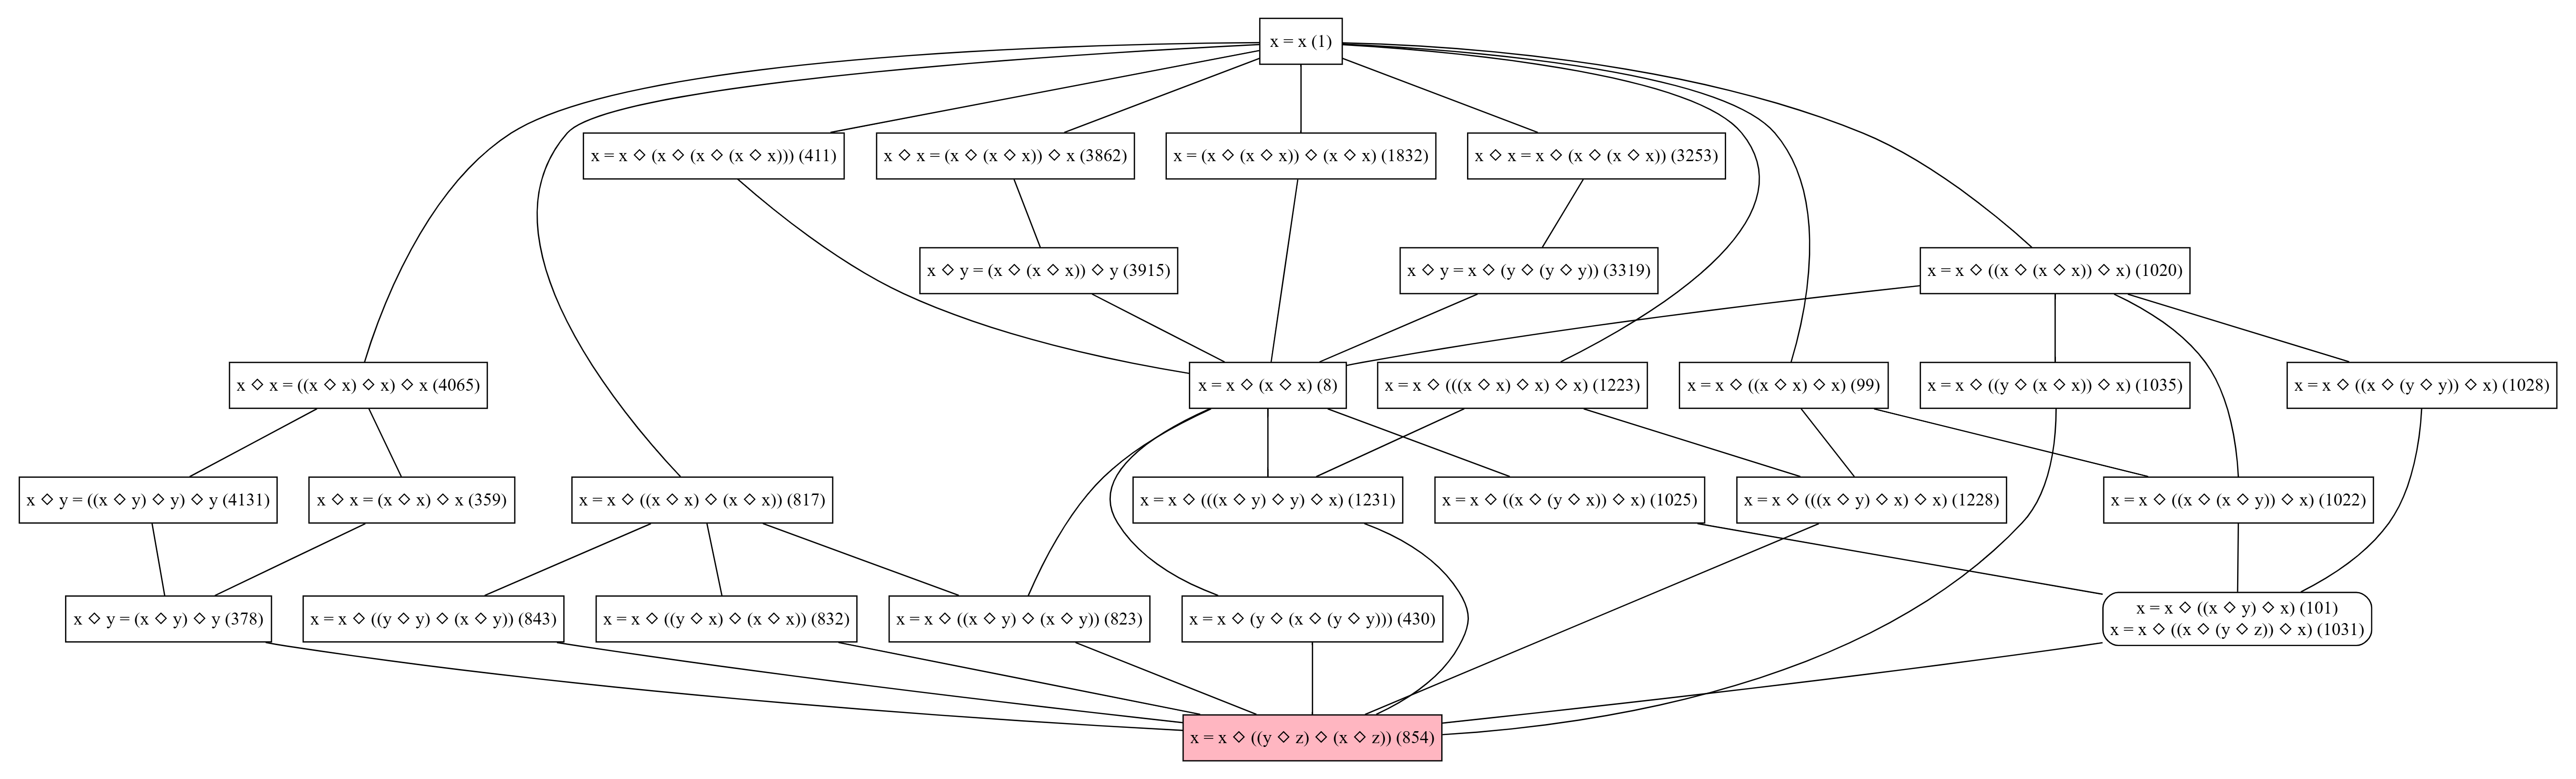
\includegraphics[width=0.85\textwidth]{854.png}
\caption{A Hasse diagram of all the equational laws implied by \Cref{eq854}.  An edge in this diagram indicates that the lower equation implies the higher one. Rounded rectangles indicate groups of equivalent laws.  This graph was produced by the visualization tool \emph{Graphiti}, which was developed for this project.}
\label{fig:854}
\end{figure}


Of the $22033636$ possible implications $E \vdash E'$, $8178279$ (or $37.12\%$) would end up being true. To establish such positive implications $E \vdash E'$, the main techniques used were as follows:

\begin{itemize}
    \item A very small number of positive implications were established and formalized by hand, mostly through direct rewriting of the laws; but this approach would not scale to the full project.
    \item Simple rewriting rules, for instance based on the observation that any law of the form $\x \formaleq f(\y,\z,\dots)$ was necessarily equivalent to the trivial law \Cref{eq2}, could already reduce the size of potential equivalence classes by a significant fraction. We discuss this method in \Cref{rewrite-sec}.
    \item The preorder axioms for $\vdash$, as well as the ``duality'' symmetry of the preorder with respect to replacing a magma operation $x \op y$ with its opposite $x \op^{\mathrm{op}} y \coloneqq y \op x$, can be used to significantly cut down on the number of implications that need to be proven explicitly; ultimately, only $10657$ ($0.05\%$) of the positive implications needed a direct proof.
    \item Automated Theorem Provers (ATP) could be deployed at extremely fast speeds to establish a complete generating set of positive implications; see \Cref{automated-sec}.
\end{itemize}

More challenging were the $13855357$ ($62.88\%$) implications that were false, $E \not \vdash E'$. Here, the range of techniques needed to refute such implications were quite varied.
\begin{itemize}
        \item Syntactic methods, such as observing an ``matching invariant'' of the law $E$ that was not shared by the law $E'$, could be used to obtain some refutations.  For instance, if both sides of $E$ had the same order, but both sides of $E'$ did not, this could be used to syntactically refute $E \vdash E'$.  Similarly, if the law $E$ was confluent, enjoyed a complete rewriting system, or otherwise permitted some understanding of the free magma associated to that law, one could decide the assertions $E \vdash E'$ for all possible laws $E'$, or at least a significant fraction of such laws.  We discuss these methods, and the extent to which they can be automated in \Cref{syntactic-sec}.
        \item Small finite magmas, which can be described explicitly by multiplication tables, could be tested by brute force computations to provide a large number of counterexamples to implications, or by ATP-assisted methods. See \Cref{finite-sec}.
        \item Linear models, in which the magma operation took the form $x \op y = ax + by$ for some (commuting or non-commuting) coefficients $a,b$, allowed for another large class of counterexamples to implications, which could be automatically scanned for either by brute force or by Grobner basis type calculations. See \Cref{linear-sec}.
        \item Translation invariant models, in which the magma operation took the form $x \op y = x + f(y-x)$ on an additive group, or $x \op y = x f(x^{-1} y)$ on a non-commutative group, reduce matters to analyzing certain functional equations; see \Cref{translation-sec}.
        \item Greedy methods, in which either the multiplication table $(x,y) \mapsto x \op y$ or the function $f$ determining a translation-invariant model are iteratively constructed by a greedy algorithm subject to a well-chosen ruleset, were effective in resolving many implications not easily disposed of by preceding methods. See \Cref{greedy-sec}.
        \item Starting with a simple base magma $M$ obeying both $E$ and $E'$, and either enlarging it to a larger magma $M' \supset M$, extending it to a magma $N$ with a projection homomorphism $\pi: N \to M$, or modifying the multiplication table on a small number of values, also proved effective when combined with greedy methods. See \Cref{modify-base}.
        \item To each equation $E$ one can associate a ``twisting semigroup'' $S_E$.  If $S_E$ is larger than $S_{E'}$, then this can often be used to disprove the implication $E \vdash E'$; see \Cref{twisting-sec}.
        \item Some \emph{ad hoc} models based on existing mathematical objects, such as infinite trees, rings of polynomials, or ``Kisielewicz models'' utilizing the prime factorization of the natural numbers, could also handle some otherwise difficult cases.  In some cases, the magma law induced some relevant and familiar structures, such as a directed graph or a partial order, which also helped guide counterexample constructions. See \Cref{adhoc-sec}.
        \item Automated theorem provers were helpful in identifying which simplifying axioms could be added to the magma without jeopardizing the ability to refute the desired implication $E \vdash E'$.
\end{itemize}

\subsection{Extensions}

While the primary objective of the ETP was being completed, some additional related results were generated as spinoffs.  Specifically:
\begin{itemize}
\item In \Cref{finite-sec} we report on a variant of the implication graph of the original set of 4692 equations, in which the magma is required to be finite.
\item In \Cref{order-5} we report on classifying which of the $57882$ distinct laws of order $5$ are equivalent to the singleton law \Cref{eq2}, either with or without the requirement that the magma be finite.
\item In \Cref{higman-neumann} we report on classifying the laws of order $8$ that are equivalent to the Higman-Neumann law \Cref{eq42323216}.
\end{itemize}

\note{Also mention ML stuff, GUI}

\section{Notation and Mathematical Foundations}\label{notation-sec}

If $M$ is a magma, we define the left and right multiplication operators $L_a, R_a \colon M \to M$ for $a \in M$ by the formula
\begin{equation}\label{left-right}
    L_x y = R_y x \coloneqq x \op y.
\end{equation}
We also define the squaring operator $S \colon M \to M$ by
\begin{equation}\label{square-def}
    Sx \coloneqq x \op x = L_x x = R_x x
\end{equation}
and the (right) cubing operator $C \colon M \to M$ by
\begin{equation}\label{cube-def}
    Cx \coloneqq Sx \op x = R_x^2 x.
\end{equation}

If $X$ is an alphabet, we let $M_X$ denote the free magma generated by $X$, thus an element of $M_X$ is either a letter in $X$, or of the form $w_1 \op w_2$ with $w_1,w_2 \in M_X$.  Every function $f \colon X \to M$ into a magma $M$ extends to a unique homomorphism $\varphi_f \colon M_X \to M$, that is to say a function for which $\varphi_f(w \op w') = \varphi_f(w) \op \varphi_f(w')$ for all $w,w' \in M_X$.  Formally, an equational law with some indeterminates in $X$ can be written as $w_1 \formaleq w_2$ for some $w_1, w_2 \in X$; a magma $M$ then obeys this law if and only if $\varphi_f(w_1) = \varphi_f(w_2)$ for all $f \colon X \to M$.  We also define the order of a word $w \in M_X$ to be the number of occurrences of $\op$ in the word, thus letters in $X$ are of order $0$, and the order of $w_1 \op w_2$ is the sum of the orders of $w_1, w_2$.

A \emph{theory} is a collection $\Gamma$ of equational laws; we say that a magma $M$ \emph{satisfies} a theory, and write $M \models \Gamma$, if every law in $\Gamma$ is obeyed by $M$.  If $E$ is an equational law, we write $\Gamma \vdash E$ if every magma that satisfies $\Gamma$ also satisfies $E$. A \emph{free magma} $M_{X,\Gamma}$ for such a theory $\Gamma$ and an alphabet $X$ is a magma satisfying $\Gamma$ together with a map $\iota_{X,\Gamma} \colon X \to M_{X,\Gamma}$ which is universal in the sense that every function $f \colon X \to M$ to a magma $M$ satisfying $\Gamma$ uniquely determines a homomorphism $\varphi_{f,\Gamma} \colon M_{X,\Gamma} \to M$ such that $\phi_{f,\Gamma} \circ \iota_{X,\Gamma} = f$.  This magma is unique up to isomorphism; a canonical way to construct it is as the quotient $M_X/\sim_\Gamma$ of the free magma $M_X$ by the equivalence relation $\sim_\Gamma$ given by declaring $w \sim_\Gamma w'$ if $\Gamma \vdash w \formaleq w'$.  If $\Gamma = \{E\}$ consists of a single law $E$, we write $M_{X,E}$, $\sim_E$, $\varphi_{f,E}$ for $M_{X,\{E\}}$, $\sim_{\{E\}}$, $\varphi_{f,\{E\}}$ respectively . \note{Give reference for free magmas relative to theories}

In general, the free magma $M_{X,\Gamma}$ is difficult to describe in a tractable form, but for some theories, one has a simple description:

\begin{example}[Commutative and associative free magma]\label{semi-group} The free magma $M_{X,\{E43, E4512\}}$ for the commutative law \eqref{eq43} and the associative law \eqref{eq4512} is the free abelian semigroup generated by $X$ (with $\iota_{X,\{E43,E4512\}}$ the obvious embedding map).
\end{example}

\begin{example}[Left-absorptive free magma]\label{left-absorb}
The free magma $M_{X,\{E4\}}$ for the left-absorptive law \eqref{eq4} is the magma with carrier $X$ and operation $x \op y = x$ (with $\iota_{X,E_4}$ the identity).
\end{example}


Every magma $M$ has an opposite $M^{\mathrm{op}}$, which has the same carrier but the opposite operation $x \op^{\mathrm{op}} y \coloneqq y \op x$.  A magma $M$ obeys an equational law $E$ if and only if its opposite $M^{\mathrm{op}}$ obeys the dual law $E^*$, defined by reversing the all operations.  For instance, the dual of
$\x \op \y \formaleq \x \op (\y \op \z)$ \eqref{eq327} is $\y \op \x \formaleq (\z \op \y) \op \x$, which in our numbering system we rewrite in normal form as $\x \op \y \formaleq (\z \op \x) \op \y$ \eqref{eq395}.

We then see that the implication graph has a duality symmetry: given two equational laws $E_1,E_2$, we have $E_1 \vdash E_2$ if and only if $E_1^* \vdash E_2^*$.

\section{Formal Foundations}

\note{TODO: expand this sketch.}

Here we describe the Lean framework used to formalize the project, covering technical issues such as:

\begin{itemize}
    \item Magma operation symbol issues
    \item Syntax (`LawX`) versus semantics (`EquationX`)
    \item "Universe hell" issues
    \item Additional verification (axiom checking, Leanchecker, etc.)
    \item Use of the `conjecture` keyword
    \item Use of namespaces to avoid collisions between contributions. (Note: we messed up with this with FreeMagma! Should have namespaced back end results as well as front end ones.)
    \item Use of Facts command to efficiently handle large numbers of anti-implications at once
\end{itemize}

Upstream contributions:

\begin{itemize}
    \item \href{https://github.com/leanprover-community/mathlib4/pulls?q=is%3Apr+is%3Abody+EquationalTheories+}{Mathlib contributions}
    \item \href{https://github.com/PatrickMassot/leanblueprint/pulls?q=is%3Apr+in%3Abody+EquationalTheories+}{LeanBlueprint contributions}
\end{itemize}


\section{Project Management}\label{project-sec}

\note{TODO: expand this sketch.}

Shreyas Srinivas and Pietro Monticone have volunteered to take the lead on this section.

Discuss topics such as:
\begin{itemize}
    \item Project generation from \href{https://github.com/pitmonticone/LeanProject}{template}
    \item Github issue management with \href{https://github.com/teorth/equational_theories/labels}{labels} and \href{https://github.com/users/teorth/projects/1}{task management dashboard}
    \item Continuous integration (builds, blueprint compilation, task status transition)
    \item Pre-push git hooks
    \item Use of blueprint (small note, see \#406: blueprint chapters should be given names for stable URLs)
    \item Use of Lean Zulip (e.g. use of polls)
\end{itemize}

Maybe give some usage statistics, e.g. drawing from \url{https://github.com/teorth/equational_theories/actions/metrics/usage}

Mention that FLT is also using a similar workflow

\subsection{Handling Scaling Issues}

Also mention some early human-managed efforts ("outstanding tasks", manually generated Hasse diagram, etc.) which suffices for the first one or two days of the project but rapidly became unable to handle the scale of the project.

Mention that some forethought in setting up a Github organizational structure with explicit admin roles etc. may have had some advantages if we had done so in the planning stages of the project, but it was workable without this structure (the main issue is that a single person - Terry - had to be the one to perform various technical admin actions).

Use of transitive reduction etc. to keep the Lean codebase manageable. Note that the project is large enough that one cannot simply accept arbitrary amounts of Lean code into the codebase, as this could make compilation times explode. Also note somewhere that transitive completion can be viewed as directed graph completion on a doubled graph consisting of laws and their formal negations.

Technical debt issues, e.g., complications stemming from an early decision to make Equations.lean and AllEquations.lean the ground truth of equations for other analysis and visualization tools, leading to the need to refactor when AllEquations.lean had to be split up for performance reasons

Note that the "blueprint" that is now standard for guiding proof formalization projects is a bit too slow to keep up with this sort of project that is oriented instead about proving new results. Often new results are stated and formalized without passing through the blueprint, which is then either updated after the fact, or not at all. So the blueprint is more of an optional auxiliary guiding tool than an essential component of the workflow.

\subsection{Other Design Considerations}

Explain what "trusting" lean really means in a large project. Highlight the kind of human issues that can interfere with this and how use of tools like external checkers and PR reviews by people maintaining the projects still matters. Provide guidelines on good practices (such as branch protection or watching out for spurious modifications in PRs, for example to the CI). Highlight the importance of following a proper process for discussing and accepting new tasks, avoiding overlaps etc. These issues are less likely to arise in projects with one clearly defined decision maker as in this case, and more likely to arise when the decision making has to be delegated to many maintainers.

Note that despite the guarantees provided by Lean, non-Lean components still contained bugs. For instance an off-by-one error in an ATP run created a large number of spurious conjectures, and some early implementations of duality reductions (external to Lean) were similarly buggy. "Unit tests", e.g., checking conjectured outputs against Lean-validated outputs, or by theoretical results such as duality symmetry, were helpful, and the Equation Explorer visualization tool also helped human collaborators detect bugs.

Meta: documenting thoughts for the future record is quite valuable. It would be extremely tedious to try to reconstruct real-time impressions long after the fact just from the github commit history and Zulip chat archive.

\subsection{Maintenance}

Describe the role of maintainers and explain why they need to be conversant in the mathematics being formalised, as well as lean. As such the role of maintainers is often akin to postdocs or assistant profs in a research group who do some research of their own, but spend much of their time to guide others in performing their tasks, the key difference being that contributors are volunteers who choose their own tasks. Explain the tasks maintainers must perform. Examples:

\begin{itemize}
\item reviewing proofs,
\item helping with proofs and theorem statements when people get stuck,
\item Offering suggestions and guidance on how to produce shorter or more elegant proofs,
\item ensuring some basic standards are met in proof blocks that make proofs robust to upstream changes,
\item Creating and maintaining CI processes.
\item responding to task requests,
\item evaluating theorem and definition formulations (for example unifying many theorem statements into one using FactsSyntax).
\item suggesting better ones where possible,
\item ensuring that there is no excessive and pointless overlap of content in different contributions (TODO: elaborate on what level of overlap was permissible and what we consider excessive).
\end{itemize}


\section{Counterexample constructions}

In this section we collect the various techniques developed in the ETP to construct counterexamples to various implications $E \vdash E'$.

\subsection{Finite magmas}\label{finite-sec}

\note{TODO: Expand this sketch}

Discuss semi-automated creation of finite counterexamples (as discussed \href{https://leanprover.zulipchat.com/#narrow/stream/458659-Equational/topic/Counterexamples.20by.20Enumerating.20Words.20in.20Quotient.20Magma}{here})

Describe various sources of example magmas used in counterexamples, including the ones listed here.

Also note some ``negative results'' - classes of finite magmas that did not yield many additional refutations, e.g. commutative 5x5 magmas.

Mention that many refutations are ``immune'' to finite models, point to \Cref{austin-sec} for details.

Using SAT solvers to find medium sized finite magmas obeying a given law? See \href{https://leanprover.zulipchat.com/#narrow/stream/458659-Equational/topic/Using.20SAT.20solvers.20for.20model.20generation}{this discussion}.

Discuss computational and memory efficiencies needed to brute force over extremely large sets of magmas. SAT solving may be a better approach past a certain size!

\subsection{Linear models}\label{linear-sec}

A fruitful source of counterexamples is the class of \emph{linear magmas}, where the carrier $M$ is a ring (which may be commutative or non-commutative, finite or infinite), and the operation $\op$ is given by $x \op y = ax + by$ for some coefficients $a,b \in M$; one can also generalize this slightly to \emph{affine magmas}, in which the operation is given by $x \op y = ax + by + c$, but for simplicity we shall focus on linear magmas here.  It is easy to see that in a linear magma, any word $w(x_1,\dots,x_n)$ of $n$ indeterminates also takes the linear form
$$ w(x_1,\dots,x_n) = \sum_{i=1}^n P_{w,i}(a,b) x_i$$
for some (possibly non-commutative) polynomial $P_{w,i}$ in $a,b$ with integer coefficients.  Thus, a linear magma will obey an equational law $w_1 \formaleq w_2$ if and only if the pair $(a,b)$ lies in the (possibly non-commutative) variety
\begin{equation}\label{variety}
  \{ (a,b) \in M \times M: P_{w_1,i}(a,b) = P_{w_2,i}(a,b) \hbox{ for all } i \}.
\end{equation}
As such, a necessary condition for such a law $w_1 \formaleq w_2$ to entail another law $w'_1 \formaleq w'_2$ is that one has the inclusion
$$ \{ (a,b) \in M \times M: P_{w_1,i}(a,b) = P_{w_2,i}(a,b) \hbox{ for all } i \} \subset
\{ (a,b) \in M \times M: P_{w'_1,i}(a,b) = P_{w'_2,i}(a,b) \hbox{ for all } i \} $$
for all rings $M$.  For commutative rings, this criterion can be checked by standard Grobner basis techniques; in the noncommutative case one can use methods such as the diamond lemma \cite{diamond-lemma}.

\begin{example}[Commutative counterexample] For the law $x = y \op (((x \op y) \op x) \op y)$ \Cref{eq1286}, the variety \Cref{variety} can be computed to be
$$ \{ (a,b) \in M \times M: 1 = a+ba^3+bab, 0 = a + ba^2 b + b^2 \}$$
while the variety for the idempotent law \Cref{eq3} is
$$ \{ (a,b) \in M: a+b=1 \}.$$
Thus to show that \Cref{eq1286} does not entail \Cref{eq3}, it suffices to locate elements $a,b$ of a ring $M$ for one has $1 = a+ba^3+bab$, $0 = a + ba^2 b + b^2$, and $a+b \neq 1$.  Here one can take a commutative example, for instance when $M = \Z/p\Z$ and $(p,a,b) = (11,1,7)$.
\end{example}

\begin{example}[Noncommutative counterexample]\label{1117-ex} For the law $x = y \op ((y \op (x \op z)) \op z)$ \Cref{eq1117}, the variety \Cref{variety} can be computed to be
$$ \{ (a,b) \in M \times M: 1 = baba, 0 = a+ba^2, 0 = bab^2 + b^2 \}$$
while the variety for $x = (x \op ((x \op x) \op x)) \op x$ \Cref{eq2441} is
$$ \{ (a,b) \in M \times M: a^2 + aba^2 + abab + ab^2 + b = 1 \}.$$
Observe that if $ba = -1$, then $(a,b)$ automatically lies in the first set, and lies in the second set if and only if $(ab+1)(b-1) = 0$.  One can then show that \Cref{eq1117} does not imply \Cref{eq2441} by setting $a = L$, $b = -R$ where $L, R$ are the left and right shift operators respectively on the ring of integer-valued sequences $\Z^\N$.  With some \emph{ad hoc} effort one can convert this example into a less linear, but simpler (and easier to formalize) example, namely the magma with carrier $\Z$ and operation $x \op y = 2x - \lfloor y/2 \rfloor$.
\end{example}

\begin{remark} As essentially observed in \cite{austin}, if there is a commutative linear counterexample to an implication $E \vdash E'$, then by the Lefschetz principle this counterexample can be realized in a finite field ${\mathbb F}_q$ for some prime power $q$ (and by the Chebotarev density theorem one can in fact take $q$ to be a prime, so that the carrier is of the form $\Z/p\Z$ for some prime $p$).  As such, we have found that an effective way to refute implications by the commutative linear magma method is to simply perform a brute force search over linear magmas $x \op y = ax + by$ in $\Z/p\Z$ for various triples $(p,a,b)$. \note{Discuss performance of this method.}

On the other hand, the refutations obtained by non-commutative linear constructions need not have a finite model.  For instance, consider the refutation $E1117 \not \vdash E2441$ from \Cref{1117-ex}.  The law \Cref{eq1117} can be rewritten as $L_y R_z L_y R_z x = x$.  This implies that $R_z$ is injective and $L_y$ is surjective for all $y,z$.  For finite magmas $M$, this then implies that the $L_y, R_z$ are in fact invertible, and hence we have also $R_z L_y R_z L_y x = x$, which implies \Cref{eq2441} by setting $x=y=z$.  Thus the refutation $E1117 \not \vdash E2441$ is ``immune'' to finite counterexamples.
\end{remark}

\begin{remark}  One can also consider nonlinear magma models, such as quadratic models $x \op y = ax^2 + bxy + cy^2 + dx + ey + f$ in a cyclic group $\Z/N\Z$.  For small values of $N$, we have found such models somewhat useful in providing additional refutations of implications $E \vdash E'$ beyond what can be achieved by the linear or affine models.  However, as the polynomials associated to a word $w(x_1,\dots,x_n)$ tend to be of high degree (exponential in the order of the word), it becomes quite rare for such models to obey a given equation $E$ when $N$ is large.
\end{remark}

\begin{remark} One can also consider the seemingly more general linear model $x \op y = ax + by$, where the carrier $M$ is now an abelian group, and $a,b$ act on $M$ by homomorphisms, that is to say that they are elements of the endomorphism ring $\mathrm{End}(M)$.  However, this leads to exactly the same varieties \Cref{variety} (where $M$ is now replaced by the endomorphism ring $\mathrm{End}(M)$) and so does not increase the power of the linear model for the purposes of refuting implications.
\end{remark}

\note{Give some statistics of what proportion of refutations can be resolved by linear models.}

On the other hand, there are certainly some refutations $E \not \vdash E'$ of implications that are ``immune'' to both commutative and non-commutative models, in the sense that all such models that obey $E$, also obey $E'$.  One such example is the refutation $E1485 \vdash E151$, which we discuss further in \Cref{twisting-sec} below.

\subsection{Translation-invariant models}\label{translation-sec}

It is natural to look for counterexamples amongst magmas that obey a large number of symmetries.  One such class of counterexamples are \emph{translation-invariant models}, in which the carrier $M$ is a group, and the left translations of this group form isomorphisms of the magma $M$.  In the case of an abelian group $M = (M,+)$, such models take the form
\begin{equation}\label{xop-add}
  x \op y = x + f(y-x)
\end{equation}
for some function $f \colon M \to M$; in the case of a non-abelian group $M = (M,\cdot)$, such models instead take the form
\begin{equation}\label{xop-mul}
x \op y = x f(x^{-1} y).
\end{equation}
For such models, the verification of an equational law in $n$ variables corresponds to a functional equation for $f$ in $n-1$ variables, as the translation symmetry allows one to normalize one variable to be the identity (say). This can simplify an implication to the point where an explicit counterexample can be found.  These functional equations are trivial to analyze when $n=1$.  For $n=2$, they are not as trivial, but still quite tractable, and has led to several refutations in practice.  The method does not appear to be particularly effective for $n>2$ due to the complexity of the functional equations.

\begin{example}[Abelian example]\label{abex}  For the law $\x \formaleq (\x \op \y) \op ((\x \op \y) \op \y)$ \Cref{eq1648}, we apply the abelian translation-invariant model \Cref{xop-add} with $y=x+h$ to obtain
\begin{align*}
  x \op y &= x + f(h) \\
  (x \op y) \op y &= x + f(h) + f(h-f(h)) \\
  (x \op y) \op ((x \op y) \op y) &= x + f(h) + f(f(h-f(h)))
\end{align*}
so that this law obeys \Cref{eq1648} if and only if the functional equation
$$f(h) + f(f(h-f(h))) = 0$$
holds for all $h \in M$.  Similarly, the law $\x \formaleq (\x \op (\x \op \y)) \op \y$ \Cref{eq206} is obeyed if and only if
$$ f(f(h)) + f(h - f(f(h))) = 0$$
for all $h \in M$.  One can now check that the function $f \colon \Z \to \Z$ defined by $f(h) \coloneqq - \mathrm{sgn}(h)$ (thus $f(h)$ equals $-1$ when $h$ is positive, $+1$ when $h$ is negative, and $0$ when $h$ is zero) obeys the first functional equation but not the second, thus establishing that $E1648 \not \vdash E206$.
\end{example}

\begin{example}[Non-abelian example]\label{trans-nonab}  We now obtain the opposite refutation $E206 \not \vdash E1648$ to \Cref{abex} using the non-abelian translation-invariant model.  By similar calculations to before, we now seek to find a function $f \colon M \to M$ on a non-abelian group $(M,\cdot)$ that obeys the functional equation
\begin{equation}\label{206-eq}
 f(f(h)) f(f(f(h))^{-1} h) = 1
\end{equation}
for all $h \in M$, but fails to obey the functional equation
\begin{equation}\label{1648-eq}
   f(h) f(f(f(h)^{-1} h)) = 1
\end{equation}
for at least one $h \in M$.  Now take $M$ to be the group generated by three generators $a,b,c$ subject to the relations $a^2=b^2=c^2=1$, or equivalently the group of reduced words in $a,b,c$ with no adjacent letters in the word equal.  We define
$$ f(1) = 1, f(a)=b, f(b) = c, f(c) = a$$
and then $f(aw)=a$ for any non-empty reduced word $w$ not starting with $a$, and similarly for $b$ and $c$.  The equation \Cref{206-eq} can be checked directly for $h=1,a,b,c$.  If $h=aw$ with $w$ non-empty, reduced, and not starting with $a$, then $f(f(h))^{-1} = f(f(h)) = b$ and $f(f(f(h))^{-1} h) = f(baw) = b$, giving \Cref{206-eq} in this case, and similarly for cyclic permutations. Meanwhile, \Cref{1648-eq} can be checked to fail for $h=a$.
\end{example}

\begin{remark}  The construction in \Cref{trans-nonab} also has the following more ``geometric'' interpretation.  The carrier $M$ can be viewed as the infinite $3$-regular tree, in which every vertex imposes a cyclic ordering on its $3$ neighbors (for instance, if we embed $M$ as a planar graph, we can use the clockwise ordering).  For $x,y \in M$, we then define $x \op y$ to equal $x$ if $x=y$.  If $y$ is instead a neighbor of $x$, we define $x \op y$ to be the next neighbor of $x$ in the cyclic ordering.  Finally, if $y$ is distance two or more from $x$, we define $x \op y$ to be the neighbor of $x$ that is closest to $y$.  One can then check that this model obeys \Cref{206-eq} but not \Cref{1648-eq}.
\end{remark}

  Some refutations $E \not \vdash E'$ are ``immune'' by translation-invariant models, in that any translation-invariant model that obeys $E$, also obeys $E'$.  One obstruction is that for such models, the squaring map $S$ is necessarily an invertible map, since $Sx = x + f(0)$ in the abelian case and $Sx = xf(1)$ in the non-abelian case. On the other hand, adding the assumption of invertibility of squares can sometimes make the implication $E \vdash E'$.  For instance, the commutative law $\x \op (\y \op \y) \formaleq (\y \op \y) \op \x$ \Cref{eq4482} for a square and an arbitrary element will imply the full commutative law \Cref{eq43} for translation-invariant models due to the surjectivity of $S$, but does not imply it in general (as one can easily see by considering models where $S$ is constant).

\subsection{The twisting semigroup}\label{twisting-sec}

Suppose one has a magma $M$ obeying a law $E$, that also enjoys some endomorphisms $T, U \colon M \to M$.  Then one can ``twist'' the operation $\op$ by $T,U$ to obtain a new magma operation
\begin{equation}\label{twist} x \op' y := Tx \op Uy.
\end{equation}
If one then tests whether this new operation $\op'$ obeys the same law $E$ as the original operation $\op$, one will find that this will be the case provided that $T,U$ obey a certain set of relations.  The semigroup generated by formal generators $\mathrm{T}, \mathrm{U}$ with these relations will be called the \emph{twisting semigroup} $\operatorname{Twist}_E$ of $E$.  This can be best illustrated with some examples.

\begin{example}  We compute the twisting semigroup of $\x \formaleq (\y \op \x) \op (\x \op (\z \op \y))$ \Cref{eq1485}.  We test this law on the operation \Cref{twist}, thus we consider whether
$$x = (y \op' x) \op' (x \op' (z \op' y))$$
holds for all $x,y,z \in M$.  Substituting in \Cref{twist} and using the homomorphism property repeatedly, this reduces to
$$x = (T^2y \op TUx) \op (UTx \op (U^2T z \op U^3y)).$$
If we impose the conditions $TU=UT$, $T^2 = U^3$, then this equation would follow from \Cref{eq1485} (with $x,y,z$ replaced with $TUx$, $T^2 y$, $U^2 Tz$ respectively).  Thus the twisting semigroup $\operatorname{Twist}_{E1485}$ of \Cref{eq1485} is generated by two generators $\mathrm{T}, \mathrm{U}$ subject to the relations $\mathrm{T} \mathrm{U}=\mathrm{U} \mathrm{T} = 1$, $\mathrm{T}^2 = \mathrm{U}^3$.  This is a cyclic group of order $5$, since the relations can be rewritten as $\mathrm{T}^5 = 1$, $\mathrm{U} = \mathrm{T}^{-1}$.

Now consider $\x \formaleq (\x \op \x) \op (\x \op \x)$ \Cref{eq151}.  Applying the same procedure, we arrive at
$$x = (T^2 x \op TUx) \op (UT x \op U^2 x)$$
so the twisting group $\operatorname{Twist}_{E151}$ is generated by two generators $\mathrm{T}, \mathrm{U}$ subject to the relations $\mathrm{T} \mathrm{U}=\mathrm{U} \mathrm{T} = \mathrm{T}^2 = \mathrm{U}^2 = 1$.  This is a cyclic group of order $2$, since the relations can be rewritten as $\mathrm{T}^2 = 1$, $\mathrm{U} = \mathrm{T}$.
\end{example}

Suppose the twisting semigroup $\operatorname{Twist}_E$ is not a quotient of $\operatorname{Twist}_{E'}$, in the sense that the relations that define $\operatorname{Twist}_{E'}$ are not obeyed by the generators of $\operatorname{Twist}_E$.  Then one can often disprove the implication $E \vdash E'$ by attempting the following procedure.
\begin{itemize}
\item First, locate a non-trivial magma $M$ obeying the law $E$.  Then the Cartesian power $M^{\operatorname{Twist}_E}$ of tuples $(x_W)_{W \in \operatorname{Twist}_E}$, with the pointwise magma operation, will also obey $E$.
\item Furthermore, this Cartesian power admits two endomorphisms $T, U$ defined by
$$ T (x_W)_{W \in \operatorname{Twist}_E} = (x_{W \mathrm{T}})_{W \in \operatorname{Twist}_E};
U (x_W)_{W \in \operatorname{Twist}_E} = (x_{W \mathrm{U}})_{W \in \operatorname{Twist}_E},$$
which obey the relations defining $\operatorname{Twist}_E$.
\item We now twist the magma operation $\op$ on $M^{\operatorname{Twist}_E}$ by $T,U$ to obtain a new magma operation $\op'$ defined by \Cref{twist}, that will still obey law $E$.
\item Because $T, U$ will not obey the relations defining $\operatorname{Twist}_{E'}$, it is highly likely that this twisted operation will not obey $E'$, thus refuting the implication $E \vdash E'$.
\end{itemize}

For instance, a non-trivial finite model for \Cref{eq1485} is given by the finite field $\mathbb{F}_2$ of two elements with the NAND operation $x \op y \coloneqq 1-xy$.  If we twist $\mathbb{F}_2^5$ by the left shift $T(x_i)_{i=1}^5 = (x_{i+1})_{i=1}^5$ and right shift $U(x_i)_{i=1}^5 = (x_{i-1})_{i=1}^5$, where we extend the indices periodically modulo $5$, then the resulting operation
$$ (x_i)_{i=1}^5 \op' (y_i)_{i=1}^5 \coloneqq (1 - x_{i+1} y_{i-1})_{i=1}^5$$
on $\mathbb{F}_2^5$ will still obey \Cref{eq1485}, but will not obey \Cref{eq151}, thus showing that $E1485 \not \vdash E151$.  This particular implication does not seem to be easily establishable by any of the other methods discussed in this paper.

\note{Report on how large the twisting semigroups are in practice, and how many implications can be refuted by this method.}


\subsection{Greedy constructions}\label{greedy-sec}

We have found \emph{greedy extension methods}, or \emph{greedy methods} for short, are a powerful way to refute implications, especially when the carrier $M$ is allowed to be infinite.  A basic implementation of this method is as follows.  To build a magma operation $\op \colon M \times M \to M$ that obeys one law $E$ but not another $E'$, one can first consider \emph{partial magma operations} $\op \colon \Omega \to M$, defined on some subset $\Omega$ of $M \times M$. Thus $x \op y$ is defined if and only if $(x,y) \in \Omega$. A magma operation is then simply a partial operation which is \emph{total} in the sense that $\Omega = M \times M$.  We say that a partial magma operation is \emph{finitely supported} if $\Omega$ is finite.

In the language of first-order logic, a partial magma operation can also be viewed as a ternary relation $R(x,y,z)$ on $M$ with the axiom that $R(x,y,z) \and R(x,y,z') \implies z=z'$ for all $x,y,z \in M$.  The support $\Omega$ is then the set of $(x,y)$ for which $R(x,y,z)$ holds for some (necessarily unique) $z$, which one can then take to be the definition of $z = x \op y$.

We say that one partial operation $\op' \colon \Omega' \to M$ \emph{extends} another $\op \colon \Omega \to M$ if $\Omega'$ contains $\Omega$, and $x \op y = x \op' y$ whenever $x \op y$ (and hence $x \op' y$) are defined. Given a sequence $\op_n \colon \Omega_n \to M$ of partial operations, each of which is an extension of the previous, we can define the \emph{direct limit} $\op_\infty \colon \bigcup_n \Omega_n \to M$ to be the partial operation defined by $x \op_\infty y \coloneqq x \op_n y$ whenever $(x,y) \in \Omega_n$.

Abstractly, the greedy algorithm strategy can now be described as follows.

\begin{theorem}[Abstract greedy algorithm]\label{greedy-abstract} Let $E,E'$ be equational laws, and let $\Gamma$ be a theory of first-order sentences regarding a  partial magma operations $\op \colon \Omega \to M$ on a carrier $M$.  Assume the following axioms:
\begin{itemize}
  \item[(i)] (Seed) There exists a finitely supported partial magma operation $\op_0 \colon \Omega_0 \to M$ satisfying $\Gamma$ that contradicts $E'$, in the sense that there is some assignment of variables in $E'$ in $M$ such that both sides of $E'$ are defined using $\op_0$, but not equal to each other.
  \item[(ii)]  (Soundness)  If $\op_n \colon \Omega_n \to M$ is a sequence of partial magma operations obeying $\Gamma$ with each $\op_{n+1}$ an extension of $\op_n$, and the direct limit $\op_\infty$ is total, then this limit obeys $E$.
  \item[(iii)] (Greedy extension)  If $\op \colon \Omega \to M$ is a finitely supported partial magma operation obeying $\Gamma$, and $a,b \in M$, then there exists a finitely supported extension $\op' \colon \Omega' \to M'$ of $\op$ to a possibly larger carrier $M'$ such that $a \op' b$ is defined.
\end{itemize}
Then $E \not \vdash E'$.
\end{theorem}

\begin{proof}  We work on the countably infinite carrier $\N$.  By embedding the finitely supported operation $\op_0$ from axiom (i) into $\N$, we can assume without loss of generality that $\op_0$ has carrier $\N$.  By similar relabeling, we can assume in (iii) that $M' = M$ when $M=\N$, since any elements of $M' \backslash \N$ that
appear in $\Omega'$ can simply be reassigned to natural numbers that did not previously appear in $\Omega$.  We well-order the pairs in $\N \times \N$ by $(a_n,b_n)$ for $n=1,2,\dots$.  Iterating (iii) starting from $\op_0$, we can thus create a sequence of finitely supported magma operations $\op_0, \op_1, \dots$ on $\N$ obeying $\Gamma$, with each $\op_{n+1}$ an extension of $\op_n$, and $a_n \op_n b_n$ defined for all $n \geq 1$.  Then the direct limit $\op_\infty$ of these operations is total, and does not obey $E'$ thanks to axiom (i).  On the other hand, by axiom (ii) it obeys $E$, and the claim follows.
\end{proof}

We refer to $\Gamma$ as the \emph{rule set} for the greedy extension method. To apply \Cref{greedy-abstract} to obtain a refutation $E \vdash E'$, we have found the following trial-and-error method to work well in practice:
\begin{itemize}
\item[1.] Start with a minimal rule set $\Gamma$ that has just enough axioms to imply the soundness property for the given hypothesis $E$.
\item[2.] Attempt to establish the greedy extension property for this rule set by setting $a \op' b$ equal to a new element $c \not \in M$, and then defining additional values of $\op'$ as necessary to recover the axioms of $\Gamma'$.
\item[3.]  If this can be done in all cases, then locate a seed $\op_0$ refuting the given target $E'$, and STOP.
\item[4.]  If there is an obstruction (often due to a ``collision'' in which a given operation $x \op' y$ is required to equal two different values), add one or more rules to $\Gamma$ to avoid this obstruction, and return to Step 2.
\end{itemize}

This method is not guaranteed to halt in finite time, as there may be increasingly lengthy sets of rules one has to add to $\Gamma$ to avoid collisions.  However, in practice we have found many of the refutations that could not be resolved by simpler techniques to be amenable to this method (or variants thereof, as discussed below).

One can automate the above procedure by using ATPs (or SAT solvers) to locate new rules that are necessary and sufficient resolve any potential collision (and which, \emph{a posteriori}, can be seen to be necessarily consequences of the law $E$).  \note{Describe performance of this automated method.  Discuss the issue that some implications required a large SAT solver calculation that was difficult to formalize efficiently in Lean, prompting human-generated simplified proofs using smaller rulesets.}

However, in some cases we have found it necessary to add ``inspired'' choices of rules that were not forced by the initial hypothesis $E$, but which simplified the analysis by removing problematic classes of collisions from consideration.  We were unable to fully automate the process of guessing such choices; however, we found ATPs very useful for testing any proposed such guess.  In particular, if an ATP was able to show that the existing ruleset, together with a proposed new rule $A$, implied $E'$, then this clearly indicated that one should not add $A$ to the rule set $\Gamma$.  Conversely, if an ATP failed to establish such an implication, this was evidence that this was a ``safe'' rule to impose.

We also found that human verification of the greedy extension property was a highly error-prone process, as the case analysis often included many delicate edge cases that were easy to overlook.  Both ATPs and the Lean formalization therefore played a crucial role in verifying the human-written greedy arguments, often revealing important gaps in those arguments that required either minor or major revisions to the rule set.


\note{Give examples}

\note{Discuss translation-invariant analogues}

\note{Discuss variants in which instead of using a single partial operation $\op: \Omega \to M$ or partial function $f$ to capture the state of a greedy process, some more complicated structure is used instead.  E.g. the Asterix construction.}

\note{Discuss the 1692 case in which one had to add an infinite tree of new values rather than a finite number.}


\subsection{Modifying base models}\label{modify-base}

\note{TODO: Expand this sketch}


\subsection{Ad hoc constructions}\label{adhoc-sec}

\note{TODO: Expand this sketch}


\section{Syntactic arguments}\label{syntactic-sec}

Many proofs or refutations of implications (or equivalences) between two equational laws $E,E'$ can be obtained from the syntactic form of the equation.  We discuss some techniques here that were useful in the ETP.

\subsection{Simple rewrites}\label{rewrite-sec}

Many equational laws $E'$ can be formally deduced from a given law $E$ by applying the Lean `rw' tactic to rewrite $E'$ repeatedly by some forward or backward application of $E$ applied to arguments that match some portion of $E$.  For instance, the commutative law \eqref{eq43} clearly implies $\x \op (\y \op \z) \formaleq (\y \op \z) \op \x$ \eqref{eq4531}
by a single such rewrite.  A brute force application of such rewrite methods is already able to directly generate about $15,000$ such implications, including many equivalences to the singleton law \eqref{eq2} and the constant law \eqref{eq46}.  After applying transitive closure, this generates about four million further such implications.

A simple observation that already generates many equivalences is that any equation of the form $\x \formaleq f(\y,\z,\dots)$ necessarily is equivalent to the trivial law $\x \formaleq \y$; similarly, an equation of the form $f(\x,\y) \formaleq g(\z,\w,\dots)$ implies $f(\x,\y) \formaleq f(\x',\y')$; and so forth. \note{Give some stats on how effective this is.}

\subsection{Matching invariants}

Fix an alphabet $X$. An \emph{matching invariant} is an assignment $I \colon M_X \to {\mathcal I}$ of an object $I(w) \in {\mathcal I}$ in some space ${\mathcal I}$ to each word $w \in M_X$ with the property that if an equational law $w_1 \formaleq w_2$ has matching invariants $I(w_1)=I(w_2)$, then the same matching $I(w'_1) = I(w'_2)$ holds for any consequence $w'_1 \formaleq w'_2$.  In particular, if one law $I(w_1)=I(w_2)$ and $I(w'_1) \neq I(w'_2)$, then the law $w_1 \formaleq w_2$ does not imply the law $w'_1 \formaleq w'_2$.

A simple example of a matching invariant is the multiplicity $(n_x)_{x \in X}$ of variables of a word: if $w_1,w_2$ have all variables $x$ appear the same number of times $n_x$ in both words, then any rewriting of a word $w$ using the law $w_1 \formaleq w_2$ will preserve this property.  Hence, if $w'_1, w'_2$ do not have the each variable appear the same number of times in both words, then $w_1 \formaleq w_2$ cannot imply $w'_1 \formaleq w'_2$.  For instance, the commutative law \eqref{eq43} cannot imply the left-absorptive law \eqref{eq4}.

One source of matching invariants comes from the free magma $M_X$ of a theory:

\begin{proposition}[Free magmas and matching invariants]\label{free-inv}  Let $\Gamma$ be a theory, and let $\iota_{X,\Gamma} \colon X \to M_{X,\Gamma}$ be the map associated to the free magma $M_{X,\Gamma}$ for that theory.  Then the map $I \colon M_X \to M_{X,\Gamma}$ defined by $I(w) \coloneqq \varphi_{\iota_{X,\Gamma}}(w)$ is an invariant.
\end{proposition}

\begin{proof}  Suppose that $w_1 \formaleq w_2$ entails $w'_1 \formaleq w'_2$, and that $I(w_1) = I(w_2)$.  For any $f \colon X \to M_{X,\Gamma}$, the two maps $\varphi_f, \varphi_{f,\Gamma} \circ \varphi_{\iota_{X,\Gamma}} \colon M_X \to M_{X,\Gamma}$ are both homomorphisms that extend $f$, hence agree by the universal property of $M_X$, as displayed by the following commutative diagram:
\[\begin{tikzcd}
	&& X \\
	\\
	{M_X} && {M_{X,\Gamma}} && {M_{X,\Gamma}}
	\arrow[hook, from=1-3, to=3-1]
	\arrow["{\iota_{X,\Gamma}}"', from=1-3, to=3-3]
	\arrow["f", from=1-3, to=3-5]
	\arrow["{I = \varphi_{\iota_{X,\Gamma}}}", from=3-1, to=3-3]
	\arrow["{\varphi_f}"', curve={height=18pt}, from=3-1, to=3-5]
	\arrow["{\varphi_{f,\Gamma}}", from=3-3, to=3-5]
\end{tikzcd}\]
In particular, the hypothesis $I(w_1)=I(w_2)$ implies that $\varphi_f(w_1) = \varphi_f(w_2)$ for all $f \colon X \to M_{X,\Gamma}$; that is to say, the magma $M_{X,\Gamma}$ obeys the law $w_1 \formaleq w_2$, and hence also $w'_1 \formaleq w'_2$ by hypothesis.  In particular, $\varphi_{\iota_{X,\Gamma}}(w'_1) = \varphi_{\iota_{X,\Gamma}}(w'_2)$, which gives $I(w'_1) = I(w'_2)$ as required.
\end{proof}

\begin{example}  If we take $\Gamma = \{E4\}$ to be the theory of the left-absorptive law \eqref{eq4} as described in \Cref{left-absorb}, then the matching invariant $I(w)$ produced by \Cref{free-inv} is the left-most letter of the alphabet $X$ appearing in the word; for instance $I((\x \op \y) \op \z) = \x$.  Thus, for example, the left-absorptive law \eqref{eq4} cannot imply the right-absorptive law \eqref{eq5}.
\end{example}

\begin{example}  If we take $\Gamma = \{E43, E4512\}$ to be the theory of the commutative law \eqref{eq43} and the associative law \eqref{eq4512}, then by \Cref{semi-group}, the associated invariant $I(w) = \sum_{x \in X} n_x e_x$ is the formal sum of all the generators $e_x$ appearing in the word $w$, in the free abelian semigroup generated by those generators.  This recovers the preceding observation that the multiplicities $(n_x)_{x \in X}$ form a matching invariant.
\end{example}

\begin{example}  Let $n \geq 1$ be a positive integer, and consider the theory $\Gamma = \{E43, E4512, E_n\}$ consisting of the previous theory $\{E43, E4512\}$ together with the order $n$ law $L_x^y x = y$.  One can check that the free magma $M_{X,\Gamma}$ can be described as the free group of exponent $n$ with generators $e_x, x \in X$, with associated map $\iota_{X,\Gamma} \colon x \mapsto e_x$.  The associated matching invariant $I(w) = \sum_{x \in X} n_x e_x$ is essentially the multiplicities $(n_x \hbox{ mod } n)_{x \in X}$ modulo $n$, which gives a slightly stronger criterion than the preceding matching invariant for refuting implications.  For example, the cubic idempotent law $\x \formaleq (\x \op x) \op \x$ \eqref{eq23}
has matching invariants $e_x = 3e_x$ in the $n=2$ case, and hence does not imply the idempotent law $\x \formaleq \x \op \x$ \eqref{eq3} since $e_x \neq 2e_x$ in the $n=2$ case.
\end{example}

\note{Give some statistics on how many refutations can be established by these methods.}

\begin{remark}  One can also obtain matching invariants from the free objects associated to theories that involve additional operations beyond the magma operation $\op$, such as an identity element or an inverse operation.  We leave the precise generalization of \Cref{free-inv} to such theories to the interested reader.
\end{remark}

\subsection{Confluence}

\note{Define a confluent law and give some examples.}

\subsection{Complete rewriting systems}

\note{Define a complete rewriting system and give some examples.}

\subsection{Unique factorization}

In general, the free magma $M_{X,E}$ for a given equational law $E$, which we can canonically define as $M_X / \sim_E$, is hard to describe explicitly; indeed, from the undecidability of implications, such a magma cannot be computably described for arbitrary $E$.  Nevertheless, for some laws it is possible to obtain some partial understanding of $M_{X,E}$ from a syntactic perspective.  For instance, if we can refute the equivalence $w'_1 \sim_E w'_2$ by constructing a counterexample magma $M$ that obeys $E$ but not $w'_1 \formaleq w'_2$, then this implies that the representatives $\iota_{X,E}(w'_1), \iota_{X,E}(w'_2)$ of  $w'_1, w'_2$ in $M_{X,E}$ are distinct.

We illustrate this approach with equations $E$ of a left-absorptive form
\begin{equation}\label{left-absorptive}
\x \formaleq \x \op f(\x,\y,\z)
\end{equation}
for some word $f(\x,\y,\z)$, which imply the right-idempotent law \eqref{eq378}.

An illustrative example is the law \eqref{eq854} depicted in Figure \ref{fig:854}. Other examples are listed in \Cref{fig:854-like}.

\begin{figure}
  \centering
  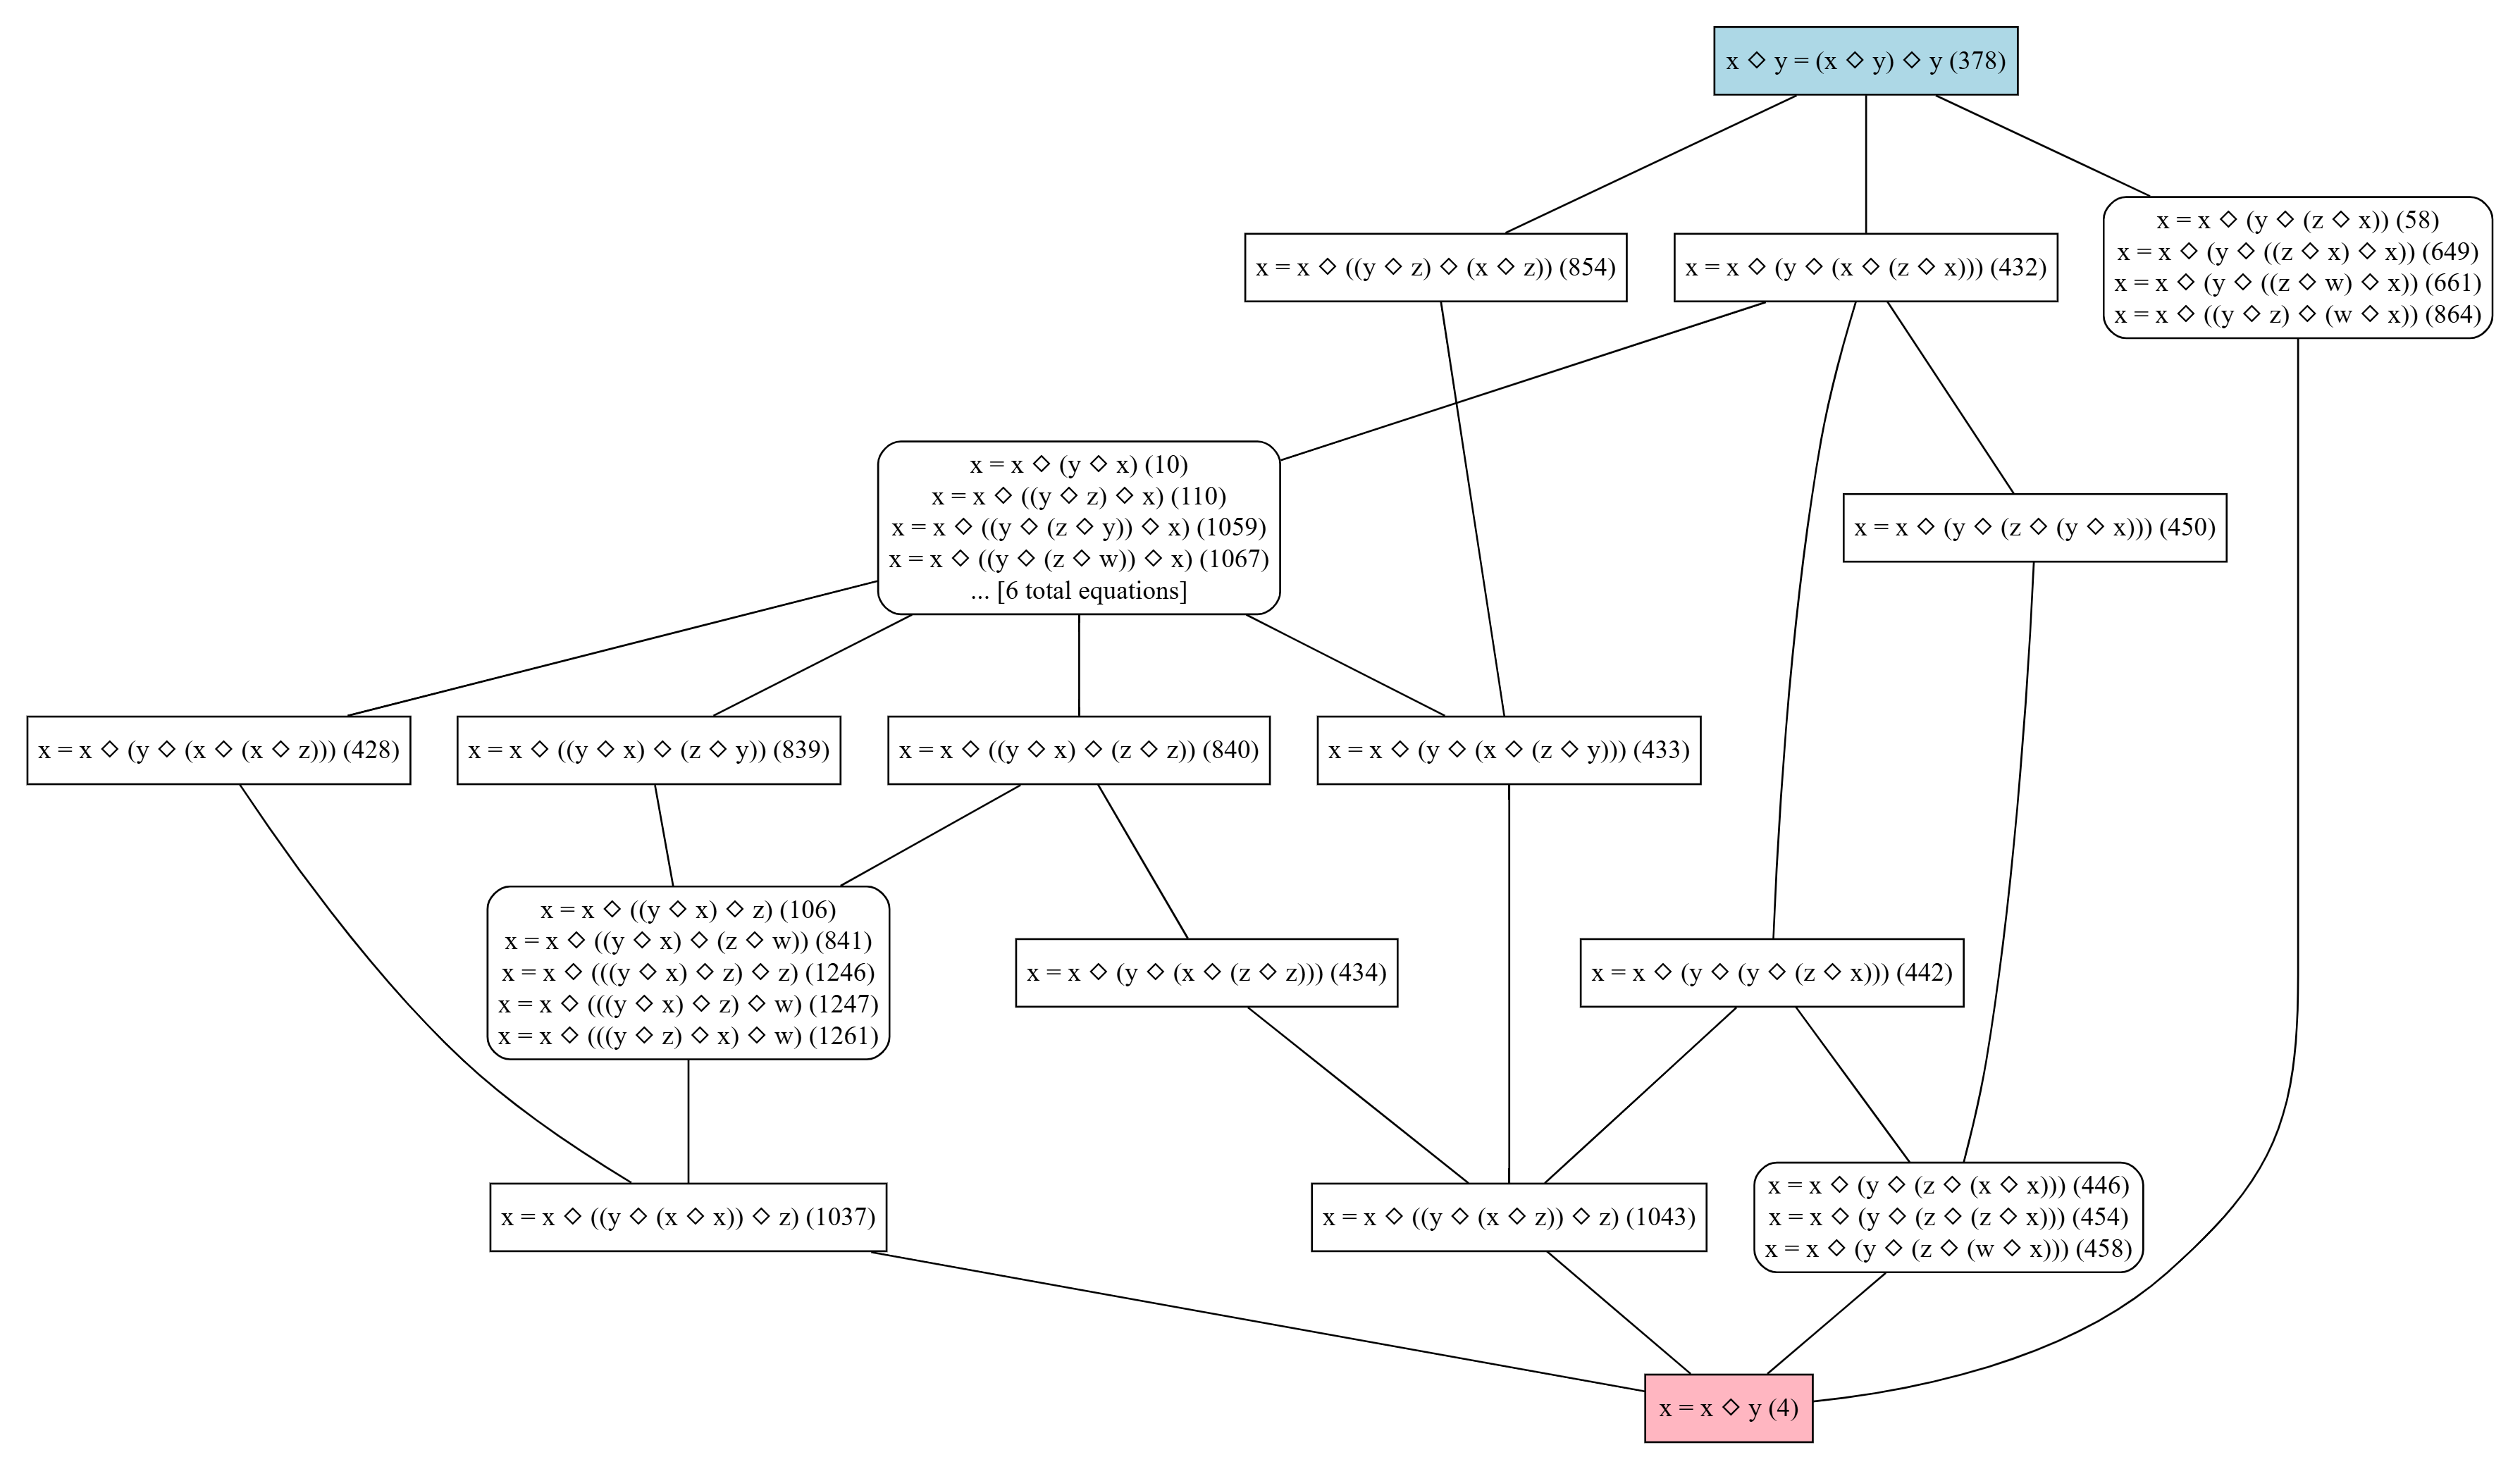
\includegraphics[width=0.85\textwidth]{854-like.png}
  \caption{Equations similar to \eqref{eq854} that are of the form \Cref{left-absorptive} (possibly involving a fourth indeterminate $\w$) and imply \eqref{eq378}.  For brevity, 70 equations equivalent to \eqref{eq4} have been omitted.}
  \label{fig:854-like}
  \end{figure}


\begin{lemma}\label{854} Equation \eqref{eq854} is of the form \Cref{left-absorptive} and implies \eqref{eq378}.
\end{lemma}

\begin{proof}  Clearly we have \Cref{left-absorptive} with $f(\x,\y,\z) \coloneqq (\y \op \z) \op (\x \op \z)$.  From \Cref{left-absorptive} we have in any magma obeying \eqref{eq854} that
$$x = x \op f(x,S^2 x,x) = x \op S(x \op S^2 x) = x \op S(x \op f(x,x,x)) = x \op Sx.$$
This implies from a further application of \Cref{left-absorptive} that
$$ y = y \op f(y,x,y) = (y \op Sy) \op ((x \op y) \op Sy) = f(x \op y, y, Sy)$$
and hence by \Cref{left-absorptive} again
$$ (x \op y) \op y = x \op y$$
giving \eqref{eq378}.
\end{proof}

Let $E$ be a law of the form \Cref{left-absorptive} that implies \eqref{eq378}. We define a directed graph $\to_E$ on words in $M_X$ by declaring $w' \to_E w$ if $w \sim_E w'' \op w'$ for some $w' \in M_X$.  By \eqref{eq378} (applied to the quotient magma $M_{X,E} = M_X/\sim_E$), this is equivalent to requiring that $w \sim_E w \op w'$. In particular, from \Cref{left-absorptive} we have $f(x,y,z) \to x$ for all $x,y,z$.  Furthermore, the relation $\to_E$ factors through $\sim_E$: if $w \sim_E \tilde w$ and $w' \sim_E \tilde w'$, then $w' \to_E w$ if and only if $\tilde w \to_E \tilde w$.

Call a word $w \in M_X$ \emph{irreducible} if it is not of the form $w = w_1 \op w_2$ with $w_2 \to_E w_1$.  We can partially understand the equivalence relation $\sim_E$ on irreducible words:

\begin{theorem}[Description of equivalence]\label{irred-desc}  Let $E$ be an equation of the form \Cref{left-absorptive}.  Let $w$ be an irreducible word, and let $w'$ be a word with $w \sim_E w'$.
  \begin{itemize}
    \item[(i)] If $w$ is a product $w = w_1 \op w_2$, then $w'$ takes the form
$$ w' = (((w'_1 \op w'_2) \op v_1) \op \dots \op v_n)$$
for some $w'_1 \sim_E w_1$, $w'_2 \sim_E w_2$, some $n \geq 0$, and some words $v_1, \dots, v_n$ such that for all $0 \leq i < n$, $v_{i+1}$ is of the form
$$ v_{i+1} \sim_E f(x_i,y_i,z_i)$$
for some $x_i, y_i, z_i$ with
$$ x_i \sim_E (((w'_1 \op w'_2) \op v_1) \op \dots \op v_i).$$
In particular, $v_{i+1} \to_E x_i$.
  \item[(ii)] Similarly, if $w \in X$ is a generator of $M_X$, then $w'$ takes the form
$$ w' = ((w \op v_1) \op \dots \op v_n)$$
for some $n \geq 0$, and some words $v_1, \dots, v_n$ such that for all $0 \leq i < n$, $v_{i+1}$ is of the form
$$ v_{i+1} \sim_E f(x_i,y_i,z_i)$$
for some $x_i, y_i, z_i$ with
$$ x_i \sim_E ((w \op v_1) \op \dots \op v_i).$$
In particular, $v_{i+1} \to_E x_i$.
\end{itemize}
Conversely, any word of the above forms is equivalent to $w$.
\end{theorem}

\begin{proof}  We just verify claim (i), as claim (ii) is similar.  The converse direction is clear from \Cref{left-absorptive} (after quotienting by $\sim_E$), so it suffices to prove the forward claim. By the Birkhoff completeness theorem, it suffices to prove that the class of words described by (i) is preserved by any term rewriting operation, in which a term in the word is replaced by an equivalent term using \Cref{left-absorptive}.  Clearly the term being rewritten is in $w'_1$ or $w'_2$ then the form of the word is preserved, and similarly if the term being rewritten is in one of the $v_i$.  The only remaining case is if we are rewriting a term of the form
$$ x_i = (((w'_1 \op w'_2) \op v_1) \op \dots \op v_i).$$
If $i>0$ we can rewrite this term down to $x_{i-1}$, and this still preserves the required form (decrementing $n$ by one).  If $i=0$ then we cannot perform such a rewriting because of the irreducibility of $w_1 \op w_2$ and hence $w'_1 \op w'_2$.  Finally, we can rewrite $x_i$ to $x_i \op v$ where $v$ is of the form
$$ v_i = f(x_i,y,z),$$
and after some relabeling we are again of the required form (now incrementing $n$ by one). This covers all possible term rewriting operations, giving the claim.
\end{proof}

Specializing to the case where $w,w'$ are both irreducible, we conclude

\begin{corollary}[Unique factorization]\label{unique factorization}  Two irreducible words $w, w'$ are equivalent if and only if they are either the same generator of $X$, or are of the form $w = w_1 \op w_2$, $w' = w'_1 \op w'_2$ with $w_1 \sim_E w'_1$ and $w_2 \sim_E w'_2$.
\end{corollary}

As an application of this corollary, we establish

\begin{proposition}[E854 does not imply E3316]\label{854-3316} Equation \eqref{eq854} does not imply \eqref{eq3316}.
\end{proposition}

\begin{proof}(Sketch)
  We work in the free group $M_X$ on two generators $X = \{\x,\y\}$.  It suffices to show that
$$  \x \op \y \not \sim_{E854} \x \op (\y \op (\x \op \y)).$$
Suppose this were not the case, then by \Cref{unique factorization} one of the following statements must hold:
\begin{itemize}
\item[(i)] $y \to_{E854} x$.
\item[(ii)] $(y \op (x \op y)) \to_{E854} x$.
\item[(iii)] $y \op (x \op y) \sim_{E854} y$.
\end{itemize}
If (i) holds, then we have $x \op y = x$ must hold in $M_X/\sim_E$, hence \eqref{eq854} would imply \eqref{eq4}.  However, it is possible to refute this implication by a finite counterexample.

Similarly, if (iii) held, then \eqref{eq854} would have to imply \eqref{eq10}, but this can also be refuted in a finite magma.

Finally, if (ii) held, then the claim
$$  x \op y \sim x \op (y \op (x \op y))$$
to refute simplifies to
$$  x \op y \sim x$$
and we are back to (i), which we already know not to be the case.
\end{proof}


\section{Automated Theorem Proving}

\note{TODO: expand this sketch}

Describe various automated theorem provers deployed in the project, with some statistics on performance:

\begin{itemize}
    \item Z3 prover
    \item Vampire
    \item More elementary substitutions
    \item egg
    \item duper
\end{itemize}

Any comparative study of semi-automated methods with fully automated ones? In principle the semi-automated approach could be more automated using a script or "agent" to call various theorem provers. See this discussion.

Draw upon the discussion here on the various ways of integrating ATPs with Lean. This project primarily used the least integrated approach, "Option 3", as it was fastest and required no dependencies on the other contributors, but it also has drawbacks.

Note: when evaluating the performance of any particular automated implication tool, we should do a fresh run on the entire base of implications, rather than rely on whatever implications produced by the tool remain in the Lean codebase by the time of writing the paper. This is because (a) many of the previous runs focused only on those implications that were not already ruled out by earlier contributions, and (b) some pruning has been applied subsequent to the initial runs to improve compilation performance. Of course, these runs would not need to be added to the (presumably optimized) codebase at that point, but would be purely for the purpose of gathering performance statistics. More discussion here.

See this discussion on the value of using different ATPs and setting run time parameters etc. at different values.

Make a note of the possible alternate strategy to prove implications outlined here.

\section{Implications for Finite Magmas}

\note{TODO: Expand this sketch}

Introduce Austin pairs.

Recap discussion from \url{https://leanprover.zulipchat.com/#narrow/channel/458659-Equational/topic/Austin.20pairs}

\section{Order 5 laws}\label{order-5}

\note{TODO: report on laws on order 5}

\section{Higman--Neumann laws}\label{higman-neumann}

\note{TODO: report on Higman--Neumann laws}

\section{AI and machine learning contributions}

\note{TODO: expand this sketch}

\begin{itemize}
\item Claude assistance in coding front ends
\item ChatGPT to guess a complete rewriting system
\item Minor use of Github Copilot etc. to autocomplete code in Lean and other languages.
\item See this discussion
\item Directed Link Prediction (DLP) on the implication graph with multiple GNN autoencoders
  (see related [Zulip topic](https://leanprover.zulipchat.com/#narrow/channel/458659-Equational/topic/Graph.20ML.3A.20Directed.20link.20prediction.20on.20the.20implication.20graph))
\end{itemize}

ML experiments to learn the implication graph

\section{User Interfaces}

A number of custom web applications were developed as part of the ETP. While many past Lean formalization projects have primarily relied on the Lean blueprint tool to organize tasks and track progress, the large volume of (transitive) implications tracked by the ETP, along with the research-oriented nature of the project, necessitated the development of custom tools to complement the blueprint tool. These web applications also made information more accessible to project participants and other interested parties, including those unfamiliar with Lean or the custom software developed for the project. The project features four primary interfaces:

\begin{enumerate}
  \item The \textbf{ETP dashboard}\footnote{\url{https://teorth.github.io/equational_theories/dashboard/}} displays the high-level overview of the project: the total number of resolved, conjectured, and unknown implications for the general and finite implication graphs. The dashboard also includes links to other tools, data, and visualizations about the implication graphs.
  \item The \textbf{Equation Explorer}\footnote{\url{https://teorth.github.io/equational_theories/implications/}} is the primary tool to navigate the implication graph. For a given equation, it display its inbound and outbound implications, as well as other members of its equivalence class. The explorer allows navigating either the general or finite implication graphs. The explorer also features custom commentary for a given equation (when available), serving as a repository for information and links. It also links to Graphiti visualizations and an example of its smallest satisfying magma, if one exists. Figure~\ref{fig:screenshot-equation-explorer} shows an example view of the explorer.
  \item \textbf{Graphiti}\footnote{\url{https://teorth.github.io/equational_theories/graphiti/}} visualizes the implication graph as a Hasse diagram, where downward edges represent subset relationships, and upward edges represent implications. Equivalence classes are collapsed into single nodes for clarity. Graphiti supports search parameters to visualize specific subsets of the graph. It can also display the entire implication graph, though the complete graph is large and challenging to navigate. Figure~\ref{fig:854-like} is an example of a Graphiti visualization.
  \item The \textbf{Finite Magma Explorer}\footnote{\url{https://teorth.github.io/equational_theories/fme/}} tests which equations a given finite magma satisfies or fails to satisfy. Users input finite magmas as Cayley tables. The tool is aware of the finite implication graph, so if an input magma witnesses an unknown refutation, it notifies the user and provides instructions for contributing the result to the GitHub repository.
\end{enumerate}

\begin{figure}
  \centering
  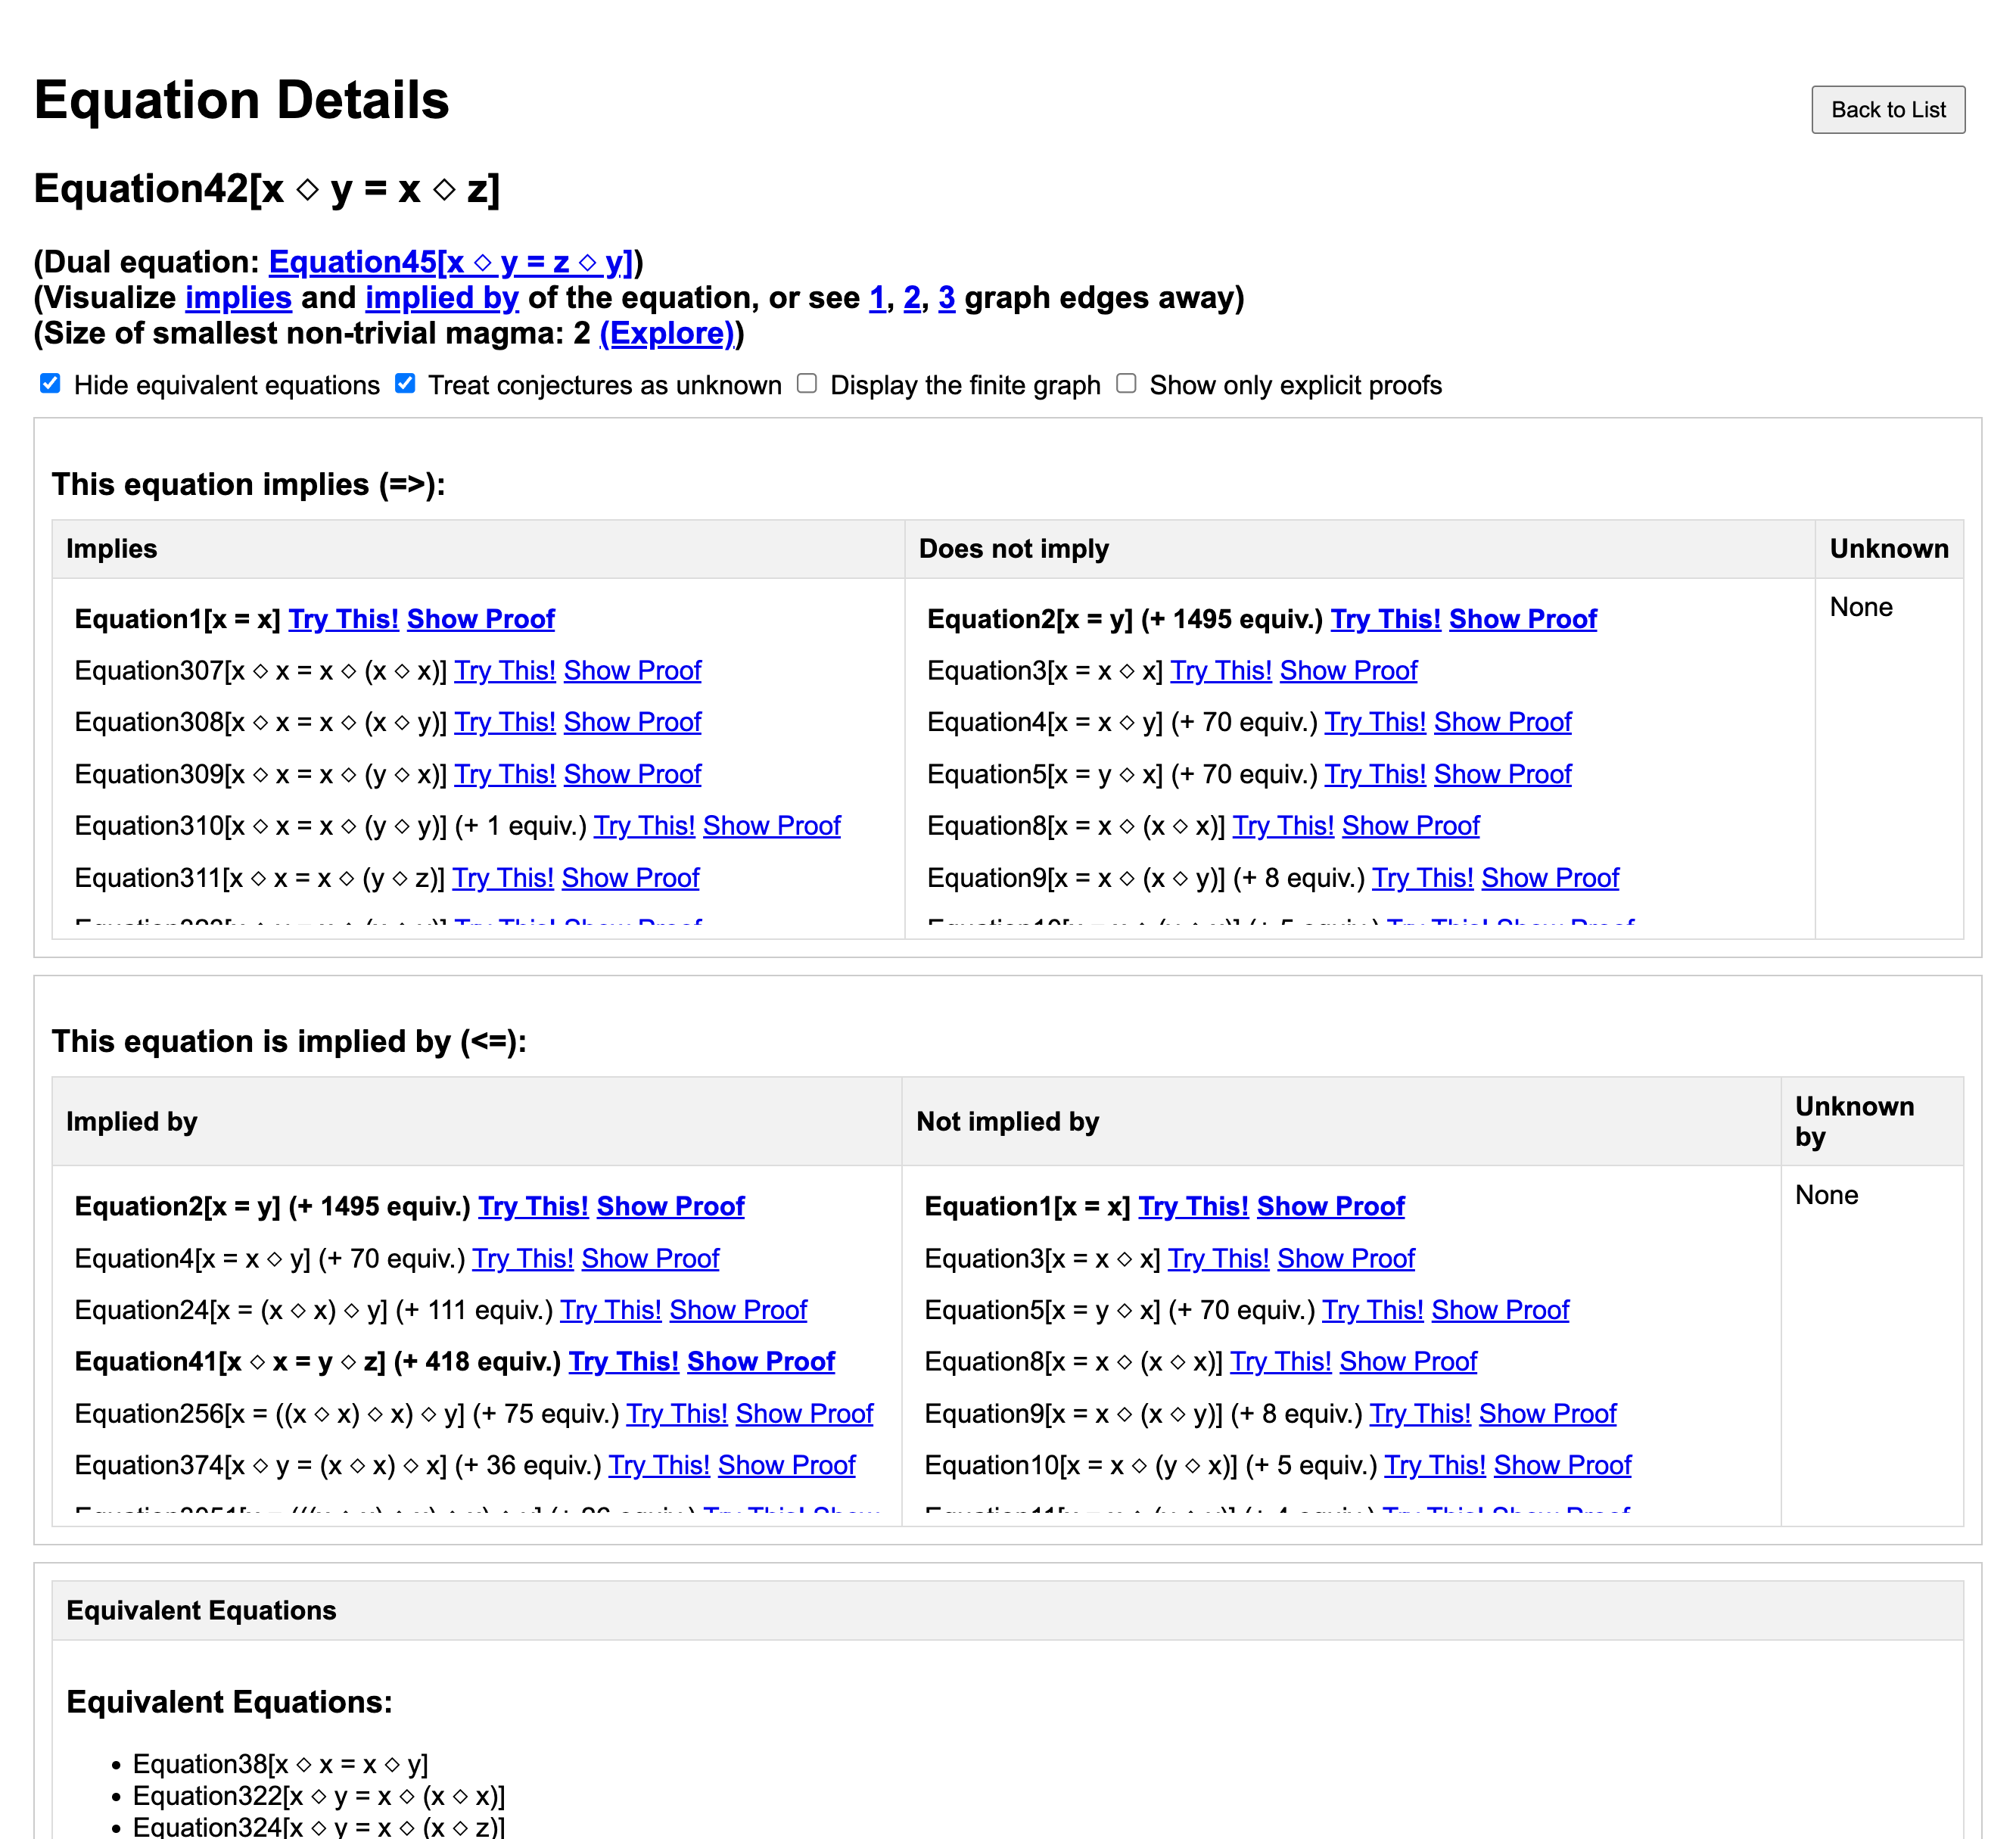
\includegraphics[width=0.85\textwidth]{GUI-equation-explorer.png}
  \caption{An example of the information displayed by the Equation Explorer for a specific equation.}
  \label{fig:screenshot-equation-explorer}
\end{figure}

The data for these tools is extracted directly from the Lean-formalized proofs in the project's GitHub repository, ensuring it always faithfully reflects the current state of progress. Additionally, the data is automatically updated with each code change using continuous integration (CI), eliminating the need for manual updates.

\section{Statistics and Experiments}

\note{TODO: Expand this sketch}

Data analysis of the implication graph:

\begin{itemize}
    \item Mention the long chain $2 \Rightarrow 5 \Rightarrow 2499 \Rightarrow 2415 \Rightarrow 238 \Rightarrow 2716 \Rightarrow 28 \Rightarrow 2973 \Rightarrow 270 \Rightarrow 3 \Rightarrow 3715 \Rightarrow 375 \Rightarrow 359 \Rightarrow 4065 \Rightarrow 1$ (discussed here).
    \item What are the "most difficult" implications?
    \item Is there a way to generate a standard test set of implication problems of various difficulty levels? Can one then use this to benchmark various automated and semi-automated methods? Challenge: how does one automatically assign a difficulty level to a given (anti-)implication?
\end{itemize}

See this for a preliminary data analysis of the impact of equation size and the number of variables.

Analyze the implication graph and discuss test sets of implication problems for benchmarking theorem provers. Challenge: How can one automatically assign a difficulty level to an implication?

\section{Data Management}

\note{TODO: expand this sketch}

Describe how data was handled during the project and how it will be managed going forward.


\section{Reflections}

\note{TODO: expand this sketch}

Testimonies from individual participants (but perhaps this is more suited for a retrospective paper). Utilize the thoughts and reflections thread.

Automation often overtook the rate of human progress, for instance in developing metatheorems. Does this create an opportunity cost? Raised as a possible discussion point here by Zoltan Kocsis.

\section{Conclusions and Future Directions}

\note{TODO: Expand this sketch}

Insights learned, future speculation. Utilize the discussion on future directions. Some ideas from that list:

\begin{itemize}
  \item A database of triple implications (EquationX and EquationY imply EquationZ) - see also this discussion.
  \item Are there any equational laws that have no non-trivial finite models, but have surjunctive models?
  \item Can we produce interesting examples of irreducible implications EquationX -> EquationY (no intermediate EquationZ can interpose)
  \item Degree of satisfiability results, e.g., if a central groupoid obeys the natural central groupoid axiom 99\% of the time, is it a natural central groupoid?
  \item Kisielewicz's question: does 5093 have any infinite models?
  \item "Insight mining" the large corpus of automated proofs that have been generated.
  \item How machine-learnable is the implication graph? (See AI/ML section)
\end{itemize}

\section*{Acknowledgments}

Thanks to \href{https://github.com/ClaudMor}{Claudio Moroni} for the exploration of directed link prediction
on the implication graph using GNN autoencoders described in \Cref{sec:dlp}.

\note{Acknowledgments to the broader Lean Zulip community and smaller contributors not listed as authors.}


\appendix

\section{Numbering system}\label{numbering-app}

In this section we record the numbering conventions we use for equational laws.

For this formal definition we use the natural numbers $0,1,2,\dots$ to represent and order indeterminate variables; however, in the main text, we use the symbols $x,y,z,w,u,v,r,s,t$ instead (and do not consider any laws with more than eight variables).

We requiring extend the ordering on indeterminate variables to a well-ordering on words $w$ in the free magma generated by these variables by declaring $w > w'$ if one of the following holds:
\begin{itemize}
    \item $w$ has a larger order than $w'$.
    \item $w = w_1 \op w_2$ and $w' = w'_1 \op w'_2$ have the same order $n \geq 1$ with $w_1 > w'_1$.
    \item $w = w_1 \op w_2$ and $w' = w'_1 \op w'_2$ have the same order $n \geq 1$ with $w_1 = w'_1$ and $w_2 > w'_2$.
\end{itemize}
Thus for instance
$$ 0 < 1 < 0 \op 0 < 0 \op 1 < 1 \op 0 $$
and
$$ 1 \op 1 < 0 \op (0 \op 0) < (0 \op 0) \op 0.$$

We similarly place a well-ordering on equational laws $w_1 \formaleq w_2$ by declaring $w_1 \formaleq w_2 > w'_1 \formaleq w'_2$ if one of the following holds:
as follows:
\begin{itemize}
\item  $w_1 \formaleq w_2$ has a longer order than $w'_1 \formaleq w'_2$.
\item If $w_1 \formaleq w_2$ has the same order as $w'_1 \formaleq w'_2$, and $w_1 > w'_1$.
\item If $w_1 \formaleq w_2$ has the same order as $w'_1 \formaleq w'_2$, $w_1 = w'_1$, and $w_2 > w'_2$.
\end{itemize}

Two equational laws are equivalent if one can be obtained from another by some combination of relabeling the variables and applying the symmetric law $w_1 \formaleq w_2 \iff w_2 \formaleq w_1$.  For instance, $(0 \op 1) \op 2 \formaleq 1$ is equivalent to $0 \formaleq (1 \op 0) \op 2$.  We then replace every equational law with their minimal element in their equivalence class, which can be viewed as the \emph{normal form} for that law; for instance, the normal form of $(0 \op 1) \op 2 \formaleq 1$ would be $0 \formaleq (1 \op 0) \op 2$.  Finally, we eliminate any law of the form $w \formaleq w$ other than $0 \formaleq 0$.  We then number the remaining equations $E1, E2, \dots$.  For instance, $E1$ is the trivial law $0 \formaleq 0$, $E2$ is the constant law $0 \formaleq 1$, $E3$ is the idempotent law $0 \formaleq 0 \op 0$, and so forth.  Lists and code for generating these equations, or the equation number attached to a given equation, can be found at the ETP repository.

The number of equations in this list of order $n=0,1,2,\dots$ is given by
$$ 2, 5, 39, 364, 4284, 57882, 888365, \dots$$
(\url{https://oeis.org/A376640}).  The number can be computed to be
$$ C_{n+1} B_{n+2}/2$$
if $n$ is odd, $2$ if $n=0$, and
$$ (C_{n+1} B_{n+2}+ C_{n/2}(2D_{n+2}-B_{n+2}))/2 - C_{n/2} B_{n/2+1}$$
if $n > 2$ is even, where $C_n, B_n$ are the Catalan and Bell numbers, and $D_n$ is the number of partitions of $[n]$ up to reflection, which for $n=0,1,2,\dots$ is
$$ 1, 1, 2, 4, 11, 32, 117, \dots$$
(\url{https://oeis.org/A103293}).  A proof of this claim can be found in the ETP blueprint.  In particular, there are $4694$ equations of order at most $4$.

Below we record some specific equations appearing in this paper, using the alphabet $x,y,z,w,u,v$ in place of $0,1,2,3,4,5,\dots$ for readability.
\begin{align}
        x &= x & \hbox{(Trivial law)} \label{eq1}\tag{E1} \\
        x &= y & \hbox{(Singleton law)} \label{eq2}\tag{E2} \\
        x &= x \op x & \hbox{(Idempotent law)} \label{eq3}\tag{E3} \\
        x &= x \op y & \hbox{(Left-absorptive law)} \label{eq4}\tag{E4} \\
        x &= y \op x & \hbox{(Right-absorptive law)} \label{eq5}\tag{E5} \\
        x &= (x \op x) \op x \label{eq23}\tag{E23} \\
        x \op x &= y \op z \label{eq41}\tag{E41} \\
        x \op y &= y \op x & \hbox{(Commutative law)} \label{eq43}\tag{E43} \\
        x \op y &= z \op w & \hbox{(Constant law)} \label{eq46}\tag{E46} \\
        x &= (y \op x) \op (x \op z) & \hbox{(Central groupoid law)} \label{eq168}\tag{E168} \\
        x \op y &= x \op (y \op z) \label{eq327}\tag{E327} \\
        x \op y &= (z \op x) \op y \label{eq395}\tag{E395} \\
        x &= y \op ( (z \op (x \op (y \op z)))) & \hbox{(Tarski's axiom)} \label{eq543}\tag{E543} \\
        x &= (y \op z) \op (y \op (x \op z)) & \hbox{(Exp. $2$ abelian groups)} \label{eq1571}\tag{E1571} \\
        x &= (y \op x) \op ((x \op z) \op z) \label{eq1689}\tag{E1689} \\
        (x \op y) \op z &= x \op (y \op z) &\hbox{(Associative law)} \label{eq4512}\tag{E4512}\\
        x \op (y \op z) &= (y \op z) \op x \label{eq4531}\tag{E4531} \\
        x &= (y \op ((x \op y) \op y)) \op (x \op (z \op y)) & \hbox{(Sheffer stroke)} \label{eq345169}\tag{E345169} \\
        x &= y \op ((((y \op y) \op x) \op z) & \hbox{(Division in groups)} \label{eq42323216}\tag{E42323216} \\
        & \quad  \op (((y \op y) \op y) \op z)) \nonumber
\end{align}

% \section{Proofs of Theoretical Results}

\note{Provide the interesting proofs mentioned in the results section, while routine proofs can refer to the blueprint or Lean.}

\section{Author Contributions}

In this section we list the authors of this paper, grant support, and their contributions to this project, using the following \href{https://credit.niso.org/}{standard CRediT categories}:

\begin{enumerate}
    \item Conceptualization: Ideas; formulation or evolution of overarching research goals and aims.
    \item Data Curation: Management activities to annotate (produce metadata), scrub data and maintain research data (including software code, where it is necessary for interpreting the data itself) for initial use and later reuse.
    \item Formal Analysis: Application of statistical, mathematical, computational, or other formal techniques to analyze or synthesize study data.
    \item Funding Acquisition: Acquisition of the financial support for the project leading to this publication.
    \item Investigation: Conducting a research and investigation process, specifically performing the experiments, or data/evidence collection.
    \item Methodology: Development or design of methodology; creation of models.
    \item Project Administration: Management and coordination responsibility for the research activity planning and execution.
    \item Resources: Provision of study materials, reagents, materials, patients, laboratory samples, animals, instrumentation, computing resources, or other analysis tools.
    \item Software: Programming, software development; designing computer programs; implementation of the computer code and supporting algorithms; testing of existing code components.
    \item Supervision: Oversight and leadership responsibility for the research activity planning and execution, including mentorship external to the core team.
    \item Validation: Verification, whether as a part of the activity or separate, of the overall replication/reproducibility of results/experiments and other research outputs.
    \item Visualization: Preparation, creation and/or presentation of the published work, specifically visualization/data presentation.
    \item Writing - Original Draft Preparation: Creation and/or presentation of the published work, specifically writing the initial draft (including substantive translation).
    \item Writing - Review and Editing: Preparation, creation and/or presentation of the published work by those from the original research group, specifically critical review, commentary or revision - including pre- or post-publication stages.
\end{enumerate}

\begin{itemize}
    \item ...
    \item Pietro Monticone, Department of Mathematics, University of Trento, pietro.monticone@studenti.unitn.it: Data Curation, Formal Analysis, Project Administration, Resources, Software, Validation, Writing - Original Draft Preparation, Writing - Review and Editing.
    \item Terence Tao, Department of Mathematics, UCLA, tao@math.ucla.edu: Conceptualization, Data Annotation, Investigation, Methodology, Project Administration, Writing - Original Draft Preparation, Writing - Review and Editing. Supported by NSF grant DMS-2347850.
    \item Harald Husum, harald.husum@gmail.com: Investigation, Software, Visualization
    \item Jérémy Scanvic, Laboratoire de Physique, École Normale Supérieure de Lyon, jeremy.scanvic@ens-lyon.fr: Validation.
    \item ...
\end{itemize}


\bibliographystyle{plain}
\bibliography{references}

\end{document}
